% 导入配置
% \documentclass[lang = cn, scheme = chinese, thmcnt = section]{elegantbook}
% elegantbook      设置elegantbook文档类
% lang = cn        设置中文环境
% scheme = chinese 设置标题为中文
% thmcnt = section 设置计数器


%% 1.封面设置

\title{Algebra Chapter 0 - Paolo Aluffi - NoteBook}                % 文档标题

\author{若水}               % 作者

\myemail{ethanmxzhou@163.com} % 邮箱

\homepage{helloethanzhou.github.io} % 主页

\date{\today}               % 日期

\extrainfo{上善若水任方圆}   % 箴言

\logo{PiCreatures_happy.pdf}        % 设置Logo

\cover{阿基米德螺旋曲线.pdf}          % 设置封面图片

% 修改标题页的色带
\definecolor{customcolor}{RGB}{135, 206, 250} 
% 定义一个名为customcolor的颜色,RGB颜色值为(135, 206, 250)

\colorlet{coverlinecolor}{customcolor}     % 将coverlinecolor颜色设置为customcolor颜色

%% 2.目录设置
\setcounter{tocdepth}{3}  % 目录深度为3

%% 3.引入宏包
\usepackage[all]{xy}
\usepackage{bbm, svg, graphicx, float, extpfeil, amsmath, amssymb, mathrsfs, mathalpha, boondox-cal, boondox-calo, hyperref, graphicx, romannum, chemarrow, booktabs, fontspec, ctex}

%% 4.定义命令
\newcommand{\N}{\mathbb{N}}            % 自然数集合
\newcommand{\R}{\mathbb{R}}            % 实数集合
\newcommand{\C}{\mathbb{C}}  		   % 复数集合
\newcommand{\Q}{\mathbb{Q}}            % 有理数集合
\newcommand{\Z}{\mathbb{Z}}            % 整数集合
\newcommand{\F}{\mathbb{F}}
\newcommand{\sub}{\subset}             % 包含
\newcommand{\im}{\text{im }}           % 像
\newcommand{\lang}{\langle}            % 左尖括号
\newcommand{\rang}{\rangle}            % 右尖括号
\newcommand{\dis}{\displaystyle}
\newcommand{\cont}{\text{cont}}
\newcommand{\cha}{\text{char}}
\newcommand{\function}[5]{
	\begin{align*}
		#1:\begin{aligned}[t]
			#2 &\longrightarrow #3\\
			#4 &\longmapsto #5
		\end{aligned}
	\end{align*}
}                                     % 函数

\newcommand{\lhdneq}{%
	\mathrel{\ooalign{$\lneq$\cr\raise.22ex\hbox{$\lhd$}\cr}}} % 真正规子群

\newcommand{\rhdneq}{%
	\mathrel{\ooalign{$\gneq$\cr\raise.22ex\hbox{$\rhd$}\cr}}} % 真正规子群

\newcommand{\upiff}{\mathrel{\rotatebox[origin=c]{90}{$\iff$}}} % 竖着的等价

\newcommand{\Rmnum}[1]{\uppercase\expandafter{\romannumeral #1}}  %定义命令输入大写罗马数字
\newcommand{\rmnum}[1]{\romannumeral #1}  %定义命令输入小写罗马数字



% \begin{document}
	
\chapter{环论$\rm\Rmnum{1}$}

\begin{figure}[H]
	\centering
	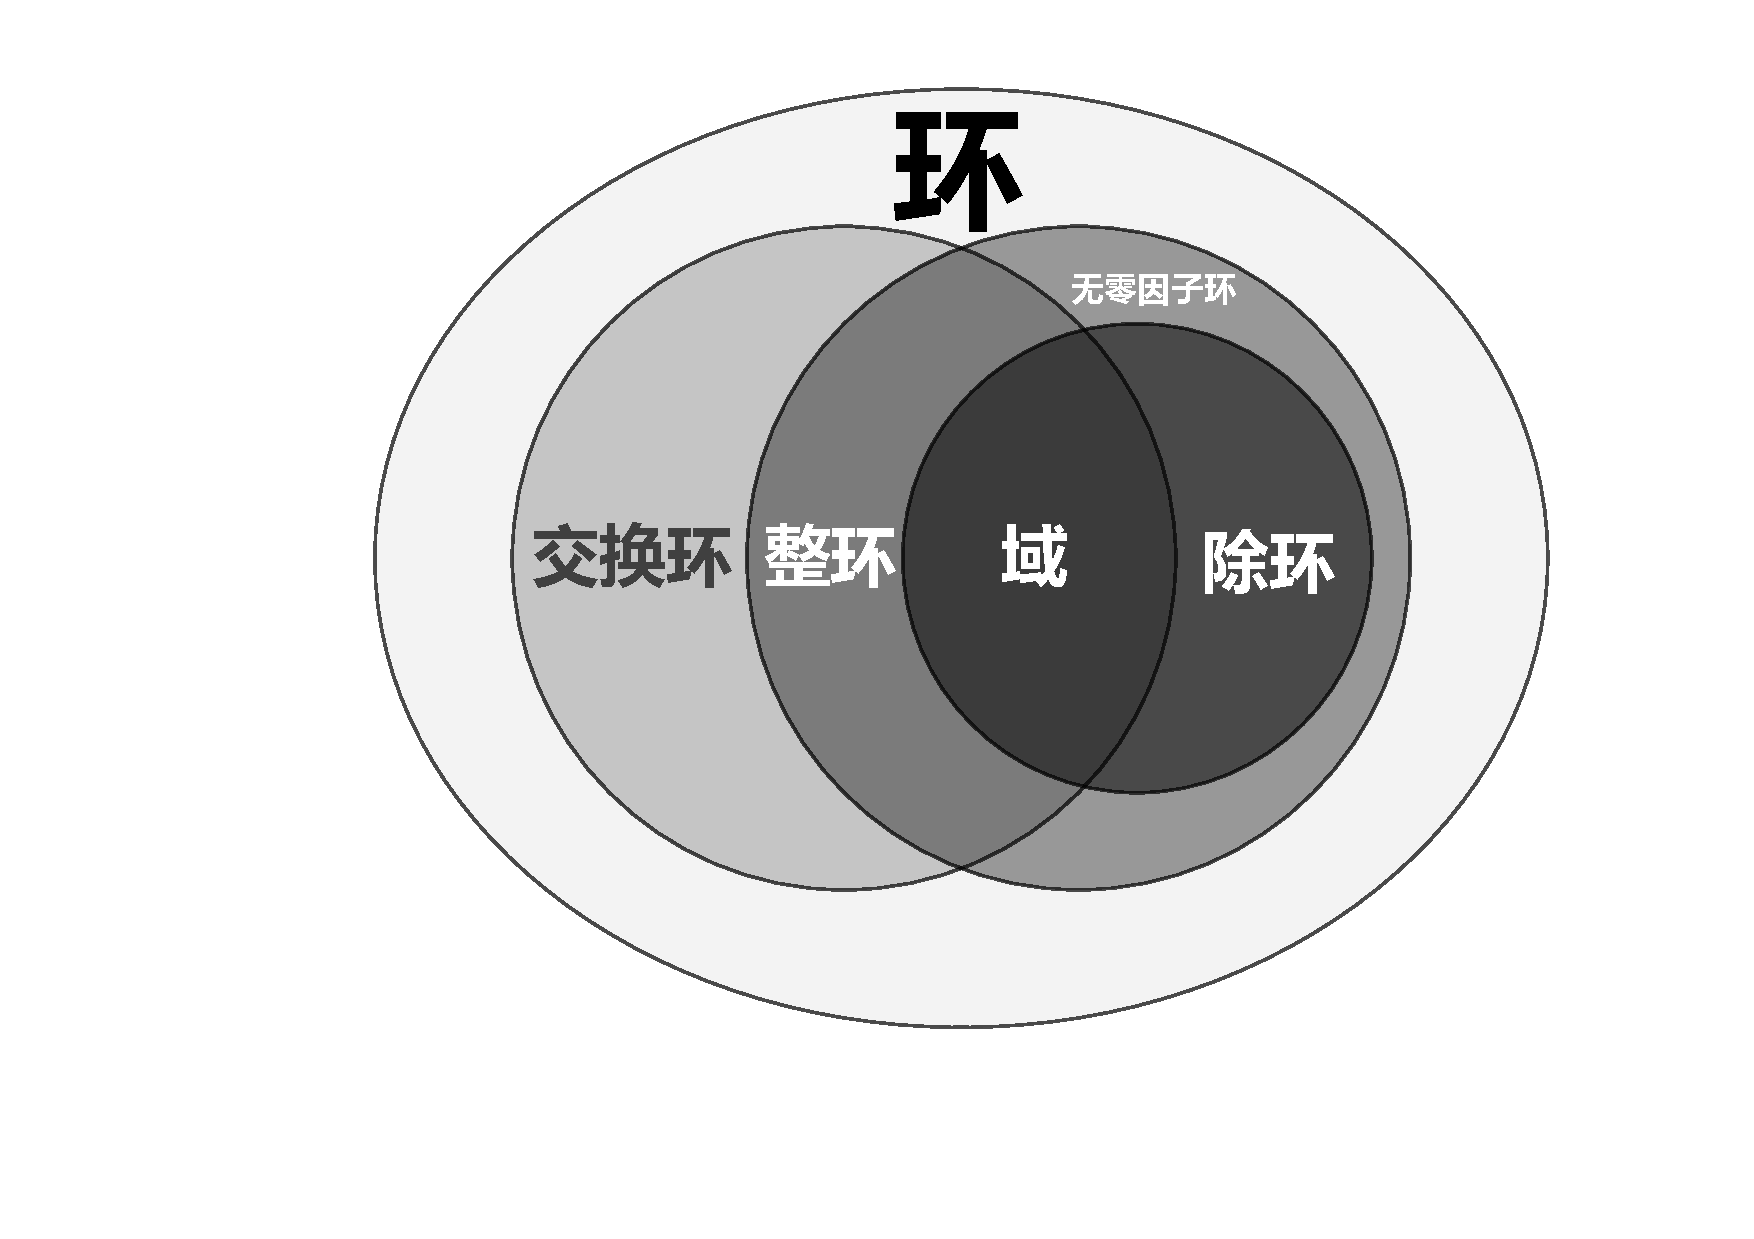
\includegraphics[scale = 0.4]{../figure/环}
	\caption{环的关系}
\end{figure}

\begin{table}[H]
	\centering
	\caption{环定义表}
	\begin{tabular}{|>{\centering\arraybackslash}m{2cm}|>{\centering\arraybackslash}m{2cm}|>{\centering\arraybackslash}m{2cm}|>{\centering\arraybackslash}m{2cm}|>{\centering\arraybackslash}m{2cm}|>{\centering\arraybackslash}m{2cm}|>{\centering\arraybackslash}m{2cm}|}
		\hline
		&      \textbf{环}      &    \textbf{交换环}    &  \textbf{无零因子环}  &     \textbf{整环}     &     \textbf{除环}     &      \textbf{域}      \\
		\hline
		\textbf{加法封闭性} & $\checkmark$ & $\checkmark$ & $\checkmark$ & $\checkmark$ & $\checkmark$ & $\checkmark$ \\
		\hline
		\textbf{乘法封闭性} & $\checkmark$ & $\checkmark$ & $\checkmark$ & $\checkmark$ & $\checkmark$ & $\checkmark$ \\
		\hline
		\textbf{加法单位元} & $\checkmark$ & $\checkmark$ & $\checkmark$ & $\checkmark$ & $\checkmark$ & $\checkmark$ \\
		\hline
		\textbf{乘法单位元} & $\checkmark$ & $\checkmark$ & $\checkmark$ & $\checkmark$ & $\checkmark$ & $\checkmark$ \\
		\hline
		\textbf{加法逆元}   & $\checkmark$ & $\checkmark$ & $\checkmark$ & $\checkmark$ & $\checkmark$ & $\checkmark$ \\
		\hline
		\textbf{加法交换律} & $\checkmark$ & $\checkmark$ & $\checkmark$ & $\checkmark$ & $\checkmark$ & $\checkmark$ \\
		\hline
		\textbf{加法结合律} & $\checkmark$ & $\checkmark$ & $\checkmark$ & $\checkmark$ & $\checkmark$ & $\checkmark$ \\
		\hline
		\textbf{乘法结合律} & $\checkmark$ & $\checkmark$ & $\checkmark$ & $\checkmark$ & $\checkmark$ & $\checkmark$ \\
		\hline
		\textbf{分配律}     & $\checkmark$ & $\checkmark$ & $\checkmark$ & $\checkmark$ & $\checkmark$ & $\checkmark$ \\
		\hline
		\textbf{非零性}     &              &              & $\checkmark$ & $\checkmark$ & $\checkmark$ & $\checkmark$ \\
		\hline
		\textbf{消去律}     &              &              & $\checkmark$ & $\checkmark$ & $\checkmark$ & $\checkmark$ \\
		\hline
		\textbf{乘法交换律} &              & $\checkmark$ &              & $\checkmark$ &              & $\checkmark$ \\
		\hline
		\textbf{乘法逆元}   &              &              &              &              & $\checkmark$ & $\checkmark$ \\
		\hline
	\end{tabular}
\end{table}

\section{环的定义}

\subsection{定义}

\begin{definition}{零环 zero-ring}
	$$
	\{0\}
	$$
\end{definition}

\begin{definition}{非零环 non-zero-ring}
	称环$(R,+,\;\cdot\;)$为非零环,如果$0\ne 1$。
\end{definition}

\begin{definition}{环 ring}
	称代数系统$(R,+,\;\cdot\;)$为环,如果加法运算$+:R\times R\to R$和乘法运算$\cdot :R\times R\to R$成立如下命题。
	\begin{enumerate}
		\item 加法单位元(addition identity element):
		$$
		\exists 0\in R,\forall r\in R,\quad 0+r=r+0=r
		$$
		\item 乘法单位元(multiplication identity element):
		$$
		\exists 1\in R,\forall r\in R,\quad 1\cdot r=r\cdot 1=r
		$$
		\item 加法逆元(addition inverse):
		$$
		\forall r\in R,\exists-r\in R,\quad r+(-r)=(-r)+r=0
		$$
		\item 加法结合律(addition associative):
		$$
		\forall r,s,t\in R,\quad (r+s)+t=r+(s+t)
		$$
		\item 乘法结合律(multiplication associative):
		$$
		\forall r,s,t\in R,\quad (r\cdot s)\cdot t=r\cdot (s\cdot t)
		$$
		\item 加法交换律(addition commutative):
		$$
		\forall r,s\in R,\quad r+s=s+r
		$$
		\item 分配律(distributive):
		\begin{align*}
			&\forall r,s,t\in R,\quad (r+s)\cdot t=r\cdot t+s\cdot t\\
			&\forall r,s,t\in R,\quad r\cdot(s+t)=r\cdot s+r\cdot t
		\end{align*}
	\end{enumerate}
\end{definition}

\begin{definition}{交换环 commutative ring}
	称代数系统$(R,+,\;\cdot\;)$为交换环,如果加法运算$+:R\times R\to R$和乘法运算$\cdot :R\times R\to R$成立如下命题。
	\begin{enumerate}
		\item 加法单位元(addition identity element):
		$$
		\exists 0\in R,\forall r\in R,\quad 0+r=r+0=r
		$$
		\item 乘法单位元(multiplication identity element):
		$$
		\exists 1\in R,\forall r\in R,\quad 1\cdot r=r\cdot 1=r
		$$
		\item 加法逆元(addition inverse):
		$$
		\forall r\in R,\exists-r\in R,\quad r+(-r)=(-r)+r=0
		$$
		\item 加法结合律(addition associative):
		$$
		\forall r,s,t\in R,\quad (r+s)+t=r+(s+t)
		$$
		\item 乘法结合律(multiplication associative):
		$$
		\forall r,s,t\in R,\quad (r\cdot s)\cdot t=r\cdot (s\cdot t)
		$$
		\item 加法交换律(addition commutative):
		$$
		\forall r,s\in R,\quad r+s=s+r
		$$
		\item 乘法交换律(multiplication commutative):
		$$
		\forall r,s\in R,\quad r\cdot s=s\cdot r
		$$
		\item 分配律(distributive):
		\begin{align*}
			&\forall r,s,t\in R,\quad (r+s)\cdot t=r\cdot t+s\cdot t\\
			&\forall r,s,t\in R,\quad r\cdot(s+t)=r\cdot s+r\cdot t
		\end{align*}
	\end{enumerate}
\end{definition}

\begin{definition}{无零因子环 without zero-divisor ring}
	称代数系统$(R,+,\;\cdot\;)$为无零因子环,如果加法运算$+:R\times R\to R$和乘法运算$\cdot :R\times R\to R$成立如下命题。
	\begin{enumerate}
		\item 加法单位元(addition identity element):
		$$
		\exists 0\in R,\forall r\in R,\quad 0+r=r+0=r
		$$
		\item 乘法单位元(multiplication identity element):
		$$
		\exists 1\in R,\forall r\in R,\quad 1\cdot r=r\cdot 1=r
		$$
		\item 加法逆元(addition inverse):
		$$
		\forall r\in R,\exists-r\in R,\quad r+(-r)=(-r)+r=0
		$$
		\item 加法结合律(addition associative):
		$$
		\forall r,s,t\in R,\quad (r+s)+t=r+(s+t)
		$$
		\item 乘法结合律(multiplication associative):
		$$
		\forall r,s,t\in R,\quad (r\cdot s)\cdot t=r\cdot (s\cdot t)
		$$
		\item 加法交换律(addition commutative):
		$$
		\forall r,s\in R,\quad r+s=s+r
		$$
		\item 消去律(cancellation):
		$$
		\forall r,s\in R,\quad r\cdot s=0\implies r=0\text{或}s=0
		$$
		\item 分配律(distributive):
		\begin{align*}
			&\forall r,s,t\in R,\quad (r+s)\cdot t=r\cdot t+s\cdot t\\
			&\forall r,s,t\in R,\quad r\cdot(s+t)=r\cdot s+r\cdot t
		\end{align*}
	\end{enumerate}
\end{definition}

\begin{definition}{整环 integral domain}
	称代数系统$(R,+,\;\cdot\;)$为整环,如果加法运算$+:R\times R\to R$和乘法$\cdot :R\times R\to R$成立如下命题。
	\begin{enumerate}
		\item 加法单位元(addition identity element):
		$$
		\exists 0\in R,\forall r\in R,\quad 0+r=r+0=r
		$$
		\item 乘法单位元(multiplication identity element):
		$$
		\exists 1\in R,\forall r\in R,\quad 1\cdot r=r\cdot 1=r
		$$
		\item 加法逆元(addition inverse):
		$$
		\forall r\in R,\exists-r\in R,\quad r+(-r)=(-r)+r=0
		$$
		\item 加法结合律(addition associative):
		$$
		\forall r,s,t\in R,\quad (r+s)+t=r+(s+t)
		$$
		\item 乘法结合律(multiplication associative):
		$$
		\forall r,s,t\in R,\quad (r\cdot s)\cdot t=r\cdot (s\cdot t)
		$$
		\item 加法交换律(addition commutative):
		$$
		\forall r,s\in R,\quad r+s=s+r
		$$
		\item 乘法交换律(multiplication commutative):
		$$
		\forall r,s\in R,\quad r\cdot s=s\cdot r
		$$
		\item 消去律(cancellation):
		$$
		\forall r,s\in R,\quad r\cdot s=0\implies r=0\text{或}s=0
		$$
		\item 分配律(distributive):
		\begin{align*}
			&\forall r,s,t\in R,\quad (r+s)\cdot t=r\cdot t+s\cdot t\\
			&\forall r,s,t\in R,\quad r\cdot(s+t)=r\cdot s+r\cdot t
		\end{align*}
	\end{enumerate}
\end{definition}

\begin{definition}{除环 division ring}
	称代数系统$(R,+,\;\cdot\;)$为除环,如果加法运算$+:R\times R\to R$和乘法$\cdot :R\times R\to R$成立如下命题。
	\begin{enumerate}
		\item 加法单位元(addition identity element):
		$$
		\exists 0\in R,\forall r\in R,\quad 0+r=r+0=r
		$$
		\item 乘法单位元(multiplication identity element):
		$$
		\exists 1\in R,\forall r\in R,\quad 1\cdot r=r\cdot 1=r
		$$
		\item 加法逆元(addition inverse):
		$$
		\forall r\in R,\exists-r\in R,\quad r+(-r)=(-r)+r=0
		$$
		\item 乘法逆元(multiplication inverse):
		$$
		\forall r\in R\setminus\{0\},\exists r^{-1}\in R,\quad r\cdot r^{-1}=r^{-1}\cdot r=1
		$$
		\item 加法结合律(addition associative):
		$$
		\forall r,s,t\in R,\quad (r+s)+t=r+(s+t)
		$$
		\item 乘法结合律(multiplication associative):
		$$
		\forall r,s,t\in R,\quad (r\cdot s)\cdot t=r\cdot (s\cdot t)
		$$
		\item 加法交换律(addition commutative):
		$$
		\forall r,s\in R,\quad r+s=s+r
		$$
		\item 分配律(distributive):
		\begin{align*}
			&\forall r,s,t\in R,\quad (r+s)\cdot t=r\cdot t+s\cdot t\\
			&\forall r,s,t\in R,\quad r\cdot(s+t)=r\cdot s+r\cdot t
		\end{align*}
	\end{enumerate}
\end{definition}

\begin{definition}{域 field}
	称代数系统$(F,+,\;\cdot\;)$为域,如果加法运算$+:F\times F\to F$和乘法运算$\cdot :F\times F\to F$成立如下命题。
	\begin{enumerate}
		\item 加法单位元(addition identity element):
		$$
		\exists 0\in F,\forall f\in F,\quad 0+f=f+0=f
		$$
		\item 乘法单位元(multiplication identity element):
		$$
		\exists 1\in F\setminus\{0\},\forall f\in F,\quad 1\cdot f=f\cdot 1=f
		$$
		\item 加法逆元(addition inverse):
		$$
		\forall f\in F,\exists-f\in F,\quad f+(-f)=(-f)+f=0
		$$
		\item 乘法逆元(multiplication inverse):
		$$
		\forall f\in F\setminus\{0\},\exists f^{-1}\in F,\quad f\cdot f^{-1}=f^{-1}\cdot f=1
		$$
		\item 加法交换律(addition commutative):
		$$
		\forall f,g\in F,\quad f+g=g+f
		$$
		\item 乘法交换律(multiplication commutative):
		$$
		\forall f,g\in F,\quad f\cdot g=g\cdot f
		$$
		\item 加法结合律(addition associative):
		$$
		\forall f,g,h\in F,\quad (f+g)+h=f+(g+h)
		$$
		\item 乘法结合律(multiplication associative):
		$$
		\forall f,g,h\in F,\quad (f\cdot g)\cdot h=f\cdot (g\cdot h)
		$$
		\item 分配律(distributive):
		\begin{align*}
			&\forall f,g,h\in F,\quad (f+g)\cdot h=f\cdot h+g\cdot h\\
			&\forall f,g,h\in F,\quad f\cdot(g+h)=f\cdot g+f\cdot h
		\end{align*}
	\end{enumerate}
\end{definition}

\begin{note}
	\begin{itemize}
		\item 环$(R,+,\;\cdot\;)$包含交换群$(R,+)$和幺半群$(R,\;\cdot\;)$,并且满足分配律。
		\item 除环$(R,+,\;\cdot\;)$包含交换群$(R,+)$和群$(R\setminus\{0\},\;\cdot\;)$,并且满足分配律。
		\item 域$(F,+,\;\cdot\;)$包含交换群$(F,+)$和交换群$(F\setminus\{0\},\;\cdot\;)$,并且满足分配律。
	\end{itemize}
\end{note}

\begin{definition}{整数环 integer ring}
	$(\Z/n\Z,+,\cdot)$,其中$[a]_n+[b]_n=[a+b]_n$,$[a]_n\cdot [b]_n=[ab]_n$。
\end{definition}

\begin{definition}{矩阵环 matrix ring}
	\begin{align*}
		&\mathfrak{gl}_n(\R)=\{ \R\text{上的} n\times n \text{可逆矩阵} \}\\
		&\mathfrak{sl}_n(\R)=\{ M\in \mathfrak{gl}_n(\R):\text{tr }(M)=0\}\\
		&\mathfrak{so}_n(\R)=\{ M\in \mathfrak{gl}_n(\R):\text{tr }(M)=1,M+M^t =0\}\\
		\\
		&\mathfrak{gl}_n(\C)=\{ \C \text{上的} n\times n \text{可逆矩阵} \}\\
		&\mathfrak{sl}_n(\C)=\{ M\in \mathfrak{gl}_n(\C):\text{tr }(M)=0\}\\
		&\mathfrak{su}_n(\C)=\{ M\in \mathfrak{gl}_n(\C):\text{tr }(M)=0,M+M^\dagger =0\}
	\end{align*}
\end{definition}

\begin{definition}{减法 subtraction}
	定义环$(R,+,\;\cdot\;)$的减法为$r-s=r+(-s)$。
\end{definition}

\begin{definition}{整数数乘 integer multiplication}
	\begin{align*}
		\Z\times R&\longrightarrow R\\
		(n,r)&\longmapsto nr=\begin{cases}
			\underbrace{r+\cdots +r}_{n\text{个}},\qquad & n\in\N^*\\
			0,\qquad & n=0\\
			(-n)r,\qquad & n\in-\N^*
		\end{cases}
	\end{align*}
\end{definition}

\begin{definition}{非负整数幂 non-negative integer power}
	\begin{align*}
		\N\times R\setminus\{(0,0)\}&\longrightarrow R\\
		(n,r)&\longmapsto r^n=\begin{cases}
			\underbrace{r\cdots r}_{n\text{个}},\qquad & n\in\N^*\\
			1,\qquad & n=0\\
		\end{cases}
	\end{align*}
\end{definition}

\begin{proposition}{环的简单性质}
	\begin{itemize}
		\item $-(-r)=r$
		\item $0r=0\cdot r=r\cdot 0=0$
		\item $-r=(-1)r=0-r=-1\cdot r=r\cdot(-1)$
		\item $(-r)\cdot(-s)=r\cdot s$
	\end{itemize}
\end{proposition}

\begin{proposition}{零环的等价条件}{零环的等价条件}
	对于环$(R,+,\;\cdot\;)$,如果$0=1$,那么$R$为零环。
\end{proposition}

\begin{proof}
	这几乎是显然的,因为
	$$
	1\cdot r=r,\qquad 0\cdot r=0
	$$
\end{proof}

\subsection{零因子与单位}

\begin{definition}{左零因子 left-zero-divisor}
	称$e\in R$为环$(R,+,\;\cdot\;)$的左零因子,如果存在非零元$u\in R$,使得成立$e\cdot u=0$;换言之
	$$
	\exists u\in R\setminus\{0\},\quad e\cdot u=0
	$$
\end{definition}

\begin{definition}{右零因子 right-zero-divisor}
	称$e\in R$为环$(R,+,\;\cdot\;)$的右零因子,如果存在非零元$v\in R$,使得成立$v\cdot e=0$;换言之
	$$
	\exists v\in R\setminus\{0\},\quad v\cdot e=0
	$$
\end{definition}

\begin{definition}{零因子 zero-divisor}
	称$e\in R$为环$(R,+,\;\cdot\;)$的零因子,如果存在非零元$r\in R$,使得成立$e\cdot r=0$或$r\cdot e=0$;换言之
	$$
	\exists r\in R\setminus\{0\},\quad e\cdot r=0\text{或}r\cdot e=0
	$$
\end{definition}

\begin{definition}{非零因子 non-zero-divisor}
	称$e\in R$为环$(R,+,\;\cdot\;)$的非零因子,如果成立如下命题之一。
	\begin{enumerate}
		\item $e$不为零因子。
		\item 对于任意非零元$r\in R$,成立$e\cdot r\ne0$且$r\cdot e\ne0$;换言之
		$$
		\forall r\in R\setminus\{0\},\quad e\cdot r\ne0\text{且}r\cdot e\ne0
		$$
		\item 对于任意$r\in R$,如果$e\cdot r=0$或$r\cdot e=0$,那么$r=0$;换言之
		$$
		\forall r\in R,\quad e\cdot r=0\text{或}r\cdot e=0\implies r=0
		$$
	\end{enumerate}
\end{definition}

\begin{definition}{无零因子环 without zero-divisor ring}
	称无非平凡零因子的非零环为无零因子环;换言之,称非零环$(R,+,\;\cdot\;)$为无零因子环,如果
	$$
	\forall r,s\in R,\quad r\cdot s=0\implies r=0\text{或}s=0
	$$
\end{definition}

\begin{definition}{整环 integral domain}
	称无零因子非零交换环为整环;换言之,称非零环$(R,+,\;\cdot\;)$为整环,如果
	\begin{align*}
		&\forall r,s\in R,\qquad r\cdot s=s\cdot r\\
		&\forall r,s\in R,\qquad r\cdot s=0\implies r=0\text{或}s=0
	\end{align*}
\end{definition}

\begin{problem}
	方程$x^2=1$在整环中仅存在根$x=\pm 1$。
\end{problem}

\begin{proof}
	$$
	x^2=1\implies (x+1)\cdot(x-1)=0\implies x+1=0\text{或}x-1=0\implies x=\pm 1
	$$
\end{proof}

\begin{proposition}{无零因子环的非零子环}{无零因子环的非零子环}
	无零因子环的非零子环为无零因子环。
\end{proposition}

\begin{proposition}{整环的非零子环}{整环的非零子环}
	整环的非零子环为整环。
\end{proposition}

\begin{proposition}
	对于环$(R,+,\;\cdot\;)$,$e\in R$不为左零因子$\iff$左乘$e$函数$R\to R$为单射。
\end{proposition}

\begin{proposition}
	整环$(R,+,\;\cdot\;)$的非零元为非零因子。
\end{proposition}

\begin{proposition}{消去律 cancellation}
	环$(R,+,\;\cdot\;)$的非零因子$e\in R$满足对于任意$r,s\in R$,成立
	$$
	e\cdot r=e\cdot s\implies r=s\\
	r\cdot e=s\cdot e\implies r=s
	$$
\end{proposition}

\begin{definition}{左单位 left-unit}
	称$e\in R$为环$(R,+,\;\cdot\;)$的左单位,如果存在$u\in R$,使得成立$e\cdot u=1$;换言之
	$$
	\exists u\in R,\quad e\cdot u=1
	$$
\end{definition}

\begin{definition}{右单位 right-unit}
	称$e\in R$为环$(R,+,\;\cdot\;)$的右单位,如果存在$v\in R$,使得成立$v\cdot e=1$;换言之
	$$
	\exists v\in R,\quad v\cdot e=1
	$$
\end{definition}

\begin{definition}{单位 unit}
	称$e\in R$为环$(R,+,\;\cdot\;)$的单位,如果存在$e^{-1}\in R$,使得成立$e\cdot e^{-1}=e^{-1}\cdot e=1$;换言之
	$$
	\exists e^{-1}\in R,\quad e\cdot e^{-1}=e^{-1}\cdot e=1
	$$
\end{definition}

\begin{definition}{单位群 group of units}
	称环$(R,+,\;\cdot\;)$的单位依乘法运算$\cdot:R\times R\to R$构成的群为单位群$(R^{\times},\;\cdot\;)$。
\end{definition}

\begin{proof}
	对于封闭性,任取单位$r,s\in R$,那么存在非零元$u,v\in R$,使得成立$u\cdot r=s\cdot v=1$,因此$u\cdot (r\cdot s)=(r\cdot s)\cdot v=1$,进而$r\cdot s$为单元。
	
	对于单位元,注意到$1\in R$为单位。
	
	对于逆元,任取单位$e\in R$,那么存在非零元$u,v\in R$,使得成立$u\cdot e=e\cdot v=1$,进而$u=u\cdot 1=u\cdot e\cdot v=1\cdot v=v$。
	
	对于结合律,这是显然的!
\end{proof}

\begin{definition}{单位的性质}
	\begin{itemize}
		\item $e\in R$为环$(R,+,\;\cdot\;)$的左单位$\iff$左乘$e$函数$R\to R$为满射。
		\item 如果$e\in R$为环$(R,+,\;\cdot\;)$的左单位,那么右乘$e$函数$R\to R$为单射,即$e$不为右零因子。
		\item 单位的加法逆元为单位。
		\item 单位的乘法逆元为单位。
	\end{itemize}
\end{definition}

\begin{proposition}
	对于环$(R,+,\;\cdot\;)$,成立
	\begin{align*}
		&r\in R\text{为左单位}\iff R=r\cdot R\\
		&r\in R\text{为右单位}\iff R=R\cdot r
	\end{align*}
\end{proposition}

\begin{proof}
	对于必要性,如果$r\in R$为左单位,那么注意到对于任意$x\in R$,成立
	$$
	x=1\cdot x=(r\cdot s)\cdot x=r\cdot (s\cdot x)\in r\cdot R
	$$
	因此$R\sub r\cdot R$,而显然$r\cdot R\sub R$,因此$R=r\cdot R$。
	
	对于充分性,如果$R=r\cdot R$,那么由$1\in R$,可知存在$s\in R$,使得成立$r\cdot s=1$,因此$r\in R$为左单位。
\end{proof}

\begin{proposition}
	对于环$(R,+,\;\cdot\;)$,如果$e\in R$为右单位,且存在至少两个左逆,那么$e$不为左零因子,但为右零因子。
\end{proposition}

\begin{proof}
	如果存在$u,v,w\in R$,使得成立$u\cdot e=1$且$v\cdot e=w\cdot e=0$,因此$v,e$之一为非零元,进而$e$为有零因子。反证,如果$e$为左零因子,那么存在非零元$r\in R$,使得成立$e\cdot r=0$,进而$r=1\cdot r=u\cdot e \cdot r=u\cdot 0=0$,矛盾!因此$e$不为左零因子。
\end{proof}

\begin{definition}{除环 division ring}
	称非零元为单位的非零环为除环;换言之,称非零环$(R,+,\;\cdot\;)$为除环,如果
	$$
	\forall r\in R\setminus\{0\},\exists r^{-1}\in R,\quad r\cdot r^{-1}=r^{-1}\cdot r=1
	$$
\end{definition}

\begin{definition}{域 field}
	交换除环为域;换言之,称非零环$(R,+,\;\cdot\;)$为域,如果
	\begin{align*}
		&\forall r,s\in R,& r &\cdot s=s\cdot r \\
		&\forall r\in R\setminus\{0\},\exists r^{-1}\in R,& r &\cdot r^{-1}=r^{-1}\cdot r=1
	\end{align*}
\end{definition}

\begin{proposition}{除环的等价条件}
	对于非零环$(R,+,\;\cdot\;)$,成立
	$$
	R\text{为除环}\iff R\text{仅存在平凡左理想}\iff R\text{仅存在平凡右理想}
	$$
\end{proposition}

\begin{proof}
	如果$R$为除环,任取$R$的非零左理想$I$,那么存在$r\in I\setminus\{0\}$,而$R$为除环,因此$1=r^{-1}\cdot r\in I$,那么$I=R$,进而$R$仅存在平凡左理想。同理对于$R$的右理想。
	
	如果$R$不为除环,那么存在$r_0\in R\setminus\{0\}$,使得对于任意$r\in R$,成立$r\cdot r_0\ne1$且$r_0\cdot r\ne 1$。由命题\ref{pro:(r)为理想},考虑左理想$R\cdot r_0$,由条件假设,$1\notin R\cdot r_0$,因此$\{0\}\subsetneq R\cdot r_0 \subsetneq R$,进而$R$存在非平凡左理想$R\cdot r_0$。同理对于$R$的右理想。
\end{proof}

\begin{proposition}{域的等价条件}{域的等价条件}
	对于非零交换环$(R,+,\;\cdot\;)$,成立
	$$
	R\text{为域}\iff R\text{仅存在平凡理想}
	$$
\end{proposition}

\begin{proof}
	如果$R$为域,任取$R$的非零理想$I$,那么存在$r\in I\setminus\{0\}$,而$R$为域,因此$1=r^{-1}\cdot r\in I$,那么$I=R$,进而$R$仅存在平凡理想。
	
	如果$R$不为域,那么存在$r_0\in R\setminus\{0\}$,使得对于任意$r\in R$,成立$r_0\cdot r\ne1$。考虑主理想$(r_0)$,由条件假设,$1\notin I$,因此$\{0\}\subsetneq (r_0) \subsetneq R$,进而$R$存在非平凡理想$(r_0)$。
\end{proof}

\begin{corollary}{}{域同态映射为单射}
	对于环同态映射$\varphi:F\to R$,如果$F$为域,那么或$R=\{0\}$,或$\varphi$为单的。
\end{corollary}

\begin{proof}
	由命题\ref{pro:核为理想},$\ker \varphi$为域$F$的理想,那么由命题\ref{pro:域的等价条件},$\ker \varphi=\{0\}$或$\ker \varphi=F$。
	
	如果$\ker\varphi=F$,那么$R=\{0\}$。
	
	如果$\ker\varphi=\{0\}$,那么$\varphi$为单的。
\end{proof}

\begin{theorem}{Wedderburn定理}
	有限除环为域。
\end{theorem}

\begin{theorem}{有限整环为域}
	有限整环为域。
\end{theorem}

\begin{proof}
	对于有限整环$(R,+,\;\cdot\;)$,任取$r\in R\setminus\{0\}$,考虑主理想$(r)$。如果$|(r)|<|R|$,那么存在互异元素$a,b\in R$,使得成立$a\cdot r=b\cdot r$。由消去律,$a=b$,矛盾!因此$|(r)|=|R|$,那么$(r)=R$。注意到$1\in R=r\cdot R$,那么存在$s\in R$,使得成立$r\cdot s=s\cdot r=1$,进而$R$为域。
\end{proof}

\begin{proposition}{循环群为整环的等价条件}{循环群为整环的等价条件}
	$$
	\Z/p\Z\text{为整环}\iff \Z/p\Z\text{为除环}\iff \Z/p\Z\text{为域}\iff p\text{为素数}
	$$
\end{proposition}

\begin{proof}
	如果$p$为素数,那么$\Z/p\Z$为非零交换环。任取$[n]_p\in\Z/p\Z\setminus\{[0]_p\}$,那么$\mathrm{gcd}(n,p)=1$。由定理\ref{thm:互素的等价条件},存在$a,b\in\Z$,使得成立
	$$
	an+bp=1\iff 
	an\equiv 1\mod p\iff 
	[an]_p=[1]_p\iff 
	[a]_p[n]_p=[1]_p
	$$
	因此$\Z/pZ$为域。
	
	如果$p$不为素数,那么存在$1<m,n<p$,使得成立$mn=p$,因此$[m]_p[n]_p=[0]_p$,但是$[m]_p\ne [0]_p$且$[n]_p\ne [0]_p$,于是$\Z_p$不成立消去律,进而$\Z_p$不为整环,亦不为除环。
\end{proof}

\begin{proposition}
	$p^2$阶除环为交换环,其中$p$为素数。
\end{proposition}

\begin{proof}
	如果$p^2$阶除环$R$不为交换群,那么$\mathrm{Cent}(R)\subsetneq R$。而$0,1\in\mathrm{Cent}(R)$,因此由命题\ref{pro:环的中心为子环},以及Lagrange定理\ref{thm:Lagrange定理},成立$|\mathrm{Cent}(R)|=p$。任取$r\in R\setminus\mathrm{Cent}(R)$,那么$\{r\}\cup \mathrm{Cent}(R)\sub \mathrm{Cent}_R(r)$,因此$|\mathrm{Cent}_R(r)|\ge p+1$,于是$|\mathrm{Cent}_R(r)|=p^2$,矛盾!
\end{proof}

\begin{definition}{四元数环 quaternion ring}
	\begin{align*}
		& \mathbb{H}=\{ a+bi+cj+dk:a,b,c,d\in \R \}\\
		& \text{其中}i,j,k\text{与}\R\text{可交换且满足}\\
		& i^2=j^2=k^2=-1,i\cdot j=-j\cdot i=k,\quad j\cdot k=-k\cdot j=i,\quad k\cdot i=-i\cdot k=j
	\end{align*}
	称$\mathbb{H}$为四元数环,$\mathbb{H}$中的元素为四元数,$\mathbb{H}$的$8$阶非交换子群
	$$
	Q_8=\{ \pm1,\pm i,\pm j,\pm k \}
	$$
	为四元数群
\end{definition}

\begin{proposition}
	四元数环$(\mathbb{H},+,\;\cdot\;)$为除环。
\end{proposition}

\begin{proof}
	$$
	(a+bi+cj+dk)\cdot\frac{a-bi-cj-dk}{a^2+b^2+c^2+d^2}=1
	$$
\end{proof}

\begin{proposition}{$\mathbb{H}$为$\mathfrak{gl}_4(\R)$的子环}
	$\mathbb{H}$为$\mathfrak{gl}_4(\R)$的子环,单的环同态映射为
	\begin{align*}
		\varphi:\begin{aligned}[t]
			\mathbb{H}&\longrightarrow\mathfrak{gl}_4(\R)\\
			a+bi+cj+dk&\longmapsto 
			\begin{pmatrix}
				a&b&c&d\\
				-b&a&-d&c\\
				-c&d&a&-b\\
				-d&-c&b&a
			\end{pmatrix}
		\end{aligned}
	\end{align*}
\end{proposition}

\begin{proposition}{$\mathbb{H}$为$\mathfrak{gl}_2(\C)$的子环}
	$\mathbb{H}$为$\mathfrak{gl}_2(\C)$的子环,单的环同态映射为
	\begin{align*}
		\psi:\begin{aligned}[t]
			\mathbb{H}&\longrightarrow\mathfrak{gl}_2(\C)\\
			a+bi+cj+dk&\longmapsto \begin{pmatrix}
				a+bi&c+di\\
				-c+di&a-bi
			\end{pmatrix}
		\end{aligned}
	\end{align*}
\end{proposition}


\subsection{幂零与Bool环}

\begin{definition}{幂零 nilpotent}
	称环$(R,+,\;\cdot\;)$的元素$r\in R$为幂零的,如果存在$n\in\N$,使得成立$r^n=0$。
\end{definition}

\begin{definition}{幂零根 nilradical}
	定义环$(R,+,\;\cdot\;)$的幂零根为
	$$
	\mathrm{Nil}(R)=\{ r\in R:\exists n\in\N^*,\text{ s.t. }r^n=0 \}
	$$
\end{definition}

\begin{definition}{即约部分 reduced part}
	称$R/\mathrm{Nil}(R)$为交换环$(R,+,\;\cdot \;)$的即约部分。
\end{definition}

\begin{definition}{即约环 reduced ring}
	称环$(R,+,\;\cdot \;)$为即约环,如果$\mathrm{Nil}(R)=\{ 0 \}$。
\end{definition}

\begin{proposition}
	$$
	[m]_n\text{为}\Z/n\Z\text{的幂零元}\iff\text{对于}n\text{的任意素因子}p\text{成立}p\mid m
	$$
\end{proposition}

\begin{proof}
	对于必要性,如果$[m]_n$为$\Z/n\Z$的幂零元素,那么存在$k\in\N$,使得成立$[m^k]_n=[0]_n$,即$n\mid m^k$。任取$n$的素因子$p$,成立$p\mid m^k$,因此$p\mid m$。
	
	对于充分性,如果对于$n$的任意素因子$p$,成立$p\mid m$,那么对$n$素因子分解$\displaystyle n=\prod_{i=1}^{r}p_i$,因此存在正整数$\{ s_i \}_{i=1}^{r}$,使得对于任意$1\le i\le r$,成立$m=s_ip_i$,注意到$\displaystyle n=\prod_{i=1}^{r}p_i\mid \prod_{i=1}^{r}s_ip_i=m^r$,因此$n\mid m^r$,进而$[m]_n$为$\Z/n\Z$的幂零元素。
\end{proof}

\begin{problem}
	构造$r,s\in R$为幂零的,但是$r+s$不为幂零的。
\end{problem}

\begin{solution}
	定义
	$$
	A=\begin{pmatrix}1&1\\-1&-1\end{pmatrix},\qquad
	B=\begin{pmatrix}1&-1\\1&-1\end{pmatrix}
	$$
	那么
	$$
	A^2=B^2=\begin{pmatrix}0&0\\0&0\end{pmatrix},\qquad 
	(A+B)^n=2^n\begin{pmatrix}1&0\\0&(-1)^n\end{pmatrix}
	$$
\end{solution}

\begin{proposition}{}{可交换幂零元的和为幂零元}
	如果$r,s\in R$为幂零的,且$r\cdot s=s\cdot r$,那么$r+s$为幂零的。
\end{proposition}

\begin{proof}
	记$m,n\in\N$满足$r^m=s^n=0$,注意到
	$$
	(r+s)^{m+n}=\sum_{k=0}^{m+n}{m+n\choose k}r^{k}\cdot s^{m+n-k}=0
	$$
\end{proof}

\begin{problem}
	构造环,使其幂零根不为理想。
\end{problem}

\begin{solution}
	$$
	A=\begin{pmatrix}1&1\\-1&-1\end{pmatrix},\qquad
	B=\begin{pmatrix}1&-1\\1&-1\end{pmatrix}
	$$
	那么
	\begin{align*}
		&A^2=B^2=\begin{pmatrix}0&0\\0&0\end{pmatrix},\quad 
		(A+B)^n=2^n\begin{pmatrix}1&0\\0&(-1)^n\end{pmatrix}\\
		&(AB)^n=2^{2n-1}\begin{pmatrix}1&-1\\-1&1\end{pmatrix},\quad
		(BA)^n=2^{2n-1}\begin{pmatrix}1&1\\1&1\end{pmatrix}
	\end{align*}
	因此矩阵环$\mathfrak{gl}_2(\R)$的幂零根不为理想,甚至不为子群。
\end{solution}

\begin{proposition}{}{交换环的幂零根为理想}
	交换环的幂零根为理想。
\end{proposition}

\begin{proof}
	对于交换环$(R,+,\;\cdot\;)$,由命题\ref{pro:可交换幂零元的和为幂零元},$\mathrm{Nil}(R)$为$R$的子群。
	
	任取$r\in R$,以及$n\in\mathrm{Nil}(R)$,那么存在$m\in \N^*$,使得成立$n^m=0$。由于
	$$
	(r\cdot n)^m=r^m\cdot n^m=r^m\cdot 0=0
	$$
	因此$r\cdot n\in\mathrm{Nil}(R)$,进而$\mathrm{Nil}(R)$为$R$的理想。
\end{proof}

\begin{proposition}{交换环的即约部分为即约环}
	交换环的即约部分为即约环;换言之,对于交换环$(R,+,\;\cdot \;)$,成立$\mathrm{Nil}(R/\mathrm{Nil}(R))=\{ \mathrm{Nil}(R) \}$
\end{proposition}

\begin{proof}
	任取$r+\mathrm{Nil}(R)\in \mathrm{Nil}(R/\mathrm{Nil}(R))$,因此存在$n$​,使得成立
	\begin{align*}
		&(r+\mathrm{Nil}(R))^n=\mathrm{Nil}(R)
		\iff r^n+\mathrm{Nil}(R)=\mathrm{Nil}(R)
		\iff r^n\in \mathrm{Nil}(R)\\
		\iff & r\in\mathrm{Nil}(R)
		\iff r+\mathrm{Nil}(R)=\mathrm{Nil}(R)
	\end{align*}
\end{proof}

\begin{definition}{Bool环 Boolean ring}
	称非零环$(R,+,\;\cdot \;)$为Bool环,如果对于任意$r\in R$,成立$r^2=r$。
\end{definition}

\begin{problem}
	对于集合$S$,定义二元运算
	\begin{align*}
		+:&\mathscr{P}(S)\times \mathscr{P}(S)\to \mathscr{P}(S)\\
		&(A,B)\mapsto (A\cup B)\setminus(A\cap B)\\
		\;\cdot\;:&\mathscr{P}(S)\times \mathscr{P}(S)\to \mathscr{P}(S)\\
		&(A,B)\mapsto A\cap B
	\end{align*}
	那么$(\mathscr{P}(S),+,\;\cdot\;)$为Bool环。
\end{problem}

\begin{proposition}{Bool环的特征}{Bool环的特征}
	Bool环的特征为$2$。
\end{proposition}

\begin{proof}
	由于$\mathsf{Ring}$范畴的初始对象为整数环$\Z$,那么对于Bool环$R\in \mathrm{Obj}(\mathsf{Ring})$,存在且存在唯一环同态映射$\varphi:\Z\to R,\quad n\mapsto n1_R$。注意到对于任意$r\in R$,成立
	$$
	2r=(2r)^2=(r+r)^2=4r^2=4r\implies 2r=0_R
	$$
	因此$\ker\varphi\supset 2\Z$。
	
	如果存在奇数$m$,使得成立$m\in\ker\varphi$,那么$\varphi(m)=0_R$,此时
	$$
	1_R=\varphi(1)=\varphi(m-(m-1))=\varphi(m)-\varphi(m-1)=0_R
	$$
	由命题\ref{pro:零环的等价条件},$R$为零环,矛盾!进而$\ker\varphi= 2\Z$,$R$的特征为$2$。
\end{proof}

\begin{proposition}{Bool环为交换环}{Bool环为交换环}
	Bool环为交换环。
\end{proposition}

\begin{proof}
	对于任意$r,s\in R$,成立
	$$
	r+s=(r+s)^2
	=r^2+r\cdot s+s\cdot r+s^2
	=r+r\cdot s+s\cdot r+s
	\implies r\cdot s+s\cdot r=0
	$$
	因此由命题\ref{pro:Bool环的特征}
	$$
	r\cdot s
	=r\cdot s+0
	=r\cdot s+r\cdot s+s\cdot r
	=2(r\cdot s)+s\cdot r
	=0+s\cdot r
	=s\cdot r
	$$
	进而Bool环$R$为交换环。
\end{proof}

\begin{proposition}
	如果整环$R$为Bool环,那么$R\cong \Z/2\Z$。
\end{proposition}

\begin{proof}
	由于$R$为Bool环,那么对于任意$r\in R$,成立$r(r-1_R)=0_R$。而$R$为整环,那么$r=0_R$,或$r=1_R$。又因为$R$不零环,那么$0_R\ne 1_R$,因此$R=\{0_R,1_R\}$,进而$R\cong \Z/2\Z$。
\end{proof}

\subsection{多项式环}

\begin{definition}{环扩张 ring extension}
	对于环$R$与$S$,称$S/R$为环扩张,如果存在单的环同态映射$\varphi:R\hookrightarrow S$。
\end{definition}

\begin{definition}{生成环}
	对于环扩张$S/R$,定义$R$关于集合$A\sub S$的生成环为
	$$
	R[A]=\bigcap_{T\supset R\cup A\text{ 为环}}T
	$$
\end{definition}

\begin{definition}{多项式环 polynomial ring}
	对于环$R$,定义其多项式环
	$$
	R[x]=\left\{ \sum_{k=0}^{n}a_kx^k:a_k\in R,n\in\N \right\}
	$$
\end{definition}

\begin{definition}{次数 degree}
	对于多项式环$R[x]$,定义多项式$\displaystyle f(x)=\sum_{k=0}^{n}a_kx^k\in R[x]$的次数为
	$$
	\deg(f(x))=\max\{ k:a_k\ne 0,0\le k \le n \}
	$$
	特别的,定义$\deg(0)=-\infty$。
\end{definition}

\begin{proposition}
	对于$f(x),g(x)\in R[x]$,成立
	$$
	\deg(f(x)+g(x))\le \max(\deg(f(x)),\deg(g(x)))
	$$
\end{proposition}

\begin{proposition}{积的次数为次数的和}{积的次数为次数的和}
	对于$f(x),g(x)\in R[x]$,如果$R$为整环,那么
	$$
	\deg(f(x)g(x))=\deg(f(x))+\deg(g(x))
	$$
\end{proposition}

\begin{proof}
	记$\displaystyle f(x)=\sum_{k=0}^{m}a_k x^k,g(x)=\sum_{k=0}^{n}b_k x^k$,其中$a_m,b_n\ne0$,由于$R$为整环,那么$a_mb_n\ne 0$,因此
	\begin{align*}
		&f(x)g(x)=\sum_{k=0}^{m+n}\sum_{i+j=k}a_i b_j x^{k}=a_mb_nx^{m+n}+\sum_{k=0}^{m+n-1}\sum_{i+j=k}a_i b_j x^{k}\\
		\implies &\deg(f(x)g(x))=m+n=\deg(f(x))+\deg(g(x))
	\end{align*}
\end{proof}

\begin{proposition}{多项式整环}{多项式整环}
	$$
	R[x]\text{为整环}\iff R\text{为整环}
	$$
\end{proposition}

\begin{proof}
	如果$R[x]$为整环,那么任取$a,b\in R$,使得成立$ab=0$,注意到$ax,bx\in R[x]$,因此$ax\cdot bx=abx^2=0$,进而$ax=0$或$bx=0$,于是$a=0$或$b=0$,那么$R$为整环。
	
	如果$R$为整环,那么任取$f(x),g(x)\in R[x]$,使得成立$f(x)g(x)=0$,由命题\ref{pro:积的次数为次数的和},可得$\deg(f(x))+\deg(g(x))=\deg(f(x)g(x))=d(0)=-\infty$,因此$f(x)=0$或$g(x)=0$,进而$R[x]$为整环。
\end{proof}

\begin{definition}{整除}
	对于多项式整环$R[x]$,称多项式$g(x)\in R[x]$整除多项式$f(x)\in R[x]$,并记作$g(x)\mid f(x)$,如果存在多项式$h(x)\in R[x]$,使得成立$f(x)=g(x)h(x)$。
\end{definition}

\begin{definition}{不可约多项式}
	对于多项式整环$R[x]$,称多项式$f(x)\in R[x]$为不可约多项式,如果$f(x)$不为常多项式,且不存在$g(x),h(x)\in R[x]$,使得成立
	$$
	f(x)=g(x)h(x),\qquad 
	\deg(g(x))<\deg(f(x)),\qquad 
	\deg(h(x))<\deg(f(x))
	$$
\end{definition}

\begin{definition}{可约多项式}
	对于多项式整环$R[x]$,称多项式$f(x)\in R[x]$为可约多项式,如果$f(x)$或为常多项式,或存在$g(x),h(x)\in R[x]$,使得成立
	$$
	f(x)=g(x)h(x),\qquad 
	\deg(g(x))<\deg(f(x)),\qquad 
	\deg(h(x))<\deg(f(x))
	$$
\end{definition}

\begin{definition}{幂级数环 ring of power series}
	对于环$R$,定义幂级数环
	$$
	R[[x]]=\left\{ \sum_{n=0}^{\infty}a_nx^n:a_n\in R \right\}
	$$
\end{definition}

\begin{problem}
	$1-x\in R[[x]]$的乘法逆元为$\displaystyle \sum_{n=0}^{\infty}{x^n}$。
\end{problem}

\begin{proposition}
	$$
	\sum_{n=0}^{\infty}a_n x^n\text{为}R[[x]]\text{的单位}\iff a_0\text{为}R\text{的单位}
	$$
\end{proposition}

\begin{proof}
	如果$\displaystyle\sum_{n=0}^{\infty}a_n x^n$为$R[[x]]$的单位,那么存在$\displaystyle\sum_{n=0}^{\infty}b_n x^n\in R[[x]]$,使得成立
	\begin{align*}
		&1=\left( \sum_{n=0}^{\infty}a_n x^n \right)\left( \sum_{n=0}^{\infty}b_n x^n \right)
		=\sum_{n=0}^{\infty}\sum_{i+j=n}a_i b_j x^{n}\implies a_0b_0=1\\
		&1=\left( \sum_{n=0}^{\infty}b_n x^n \right)\left( \sum_{n=0}^{\infty}a_n x^n \right)
		=\sum_{n=0}^{\infty}\sum_{i+j=n}a_i b_j x^{n}\implies b_0a_0=1
	\end{align*}
	因此$a_0\in R$为单位。
	
	如果$a_0$为$R$的单位,那么存在$b_0,c_0\in R$,使得成立$a_0b_0=c_0a_0=1$,递归定义
	$$
	b_{n}=-c_0\sum_{i=1}^{n}a_ib_{n-i},\qquad c_n=-\sum_{i=1}^{n}c_{n-i}a_i\cdot b_0,\qquad n\in\N^*
	$$
	那么对于任意$n\in\N^*$,成立$\displaystyle \sum_{i+j=n}a_i b_j x^{n}=\sum_{i+j=n}c_i a_j x^{n}=0$​,进而
	\begin{align*}
		&\left( \sum_{n=0}^{\infty}a_n x^n \right)\left( \sum_{n=0}^{\infty}b_n x^n \right)
		=\sum_{n=0}^{\infty}\sum_{i+j=n}a_i b_j x^{n}=a_0b_0+\sum_{n=1}^{\infty}\sum_{i+j=n}a_i b_j x^{n}=1\\
		&\left( \sum_{n=0}^{\infty}c_n x^n \right)\left( \sum_{n=0}^{\infty}a_n x^n \right)
		=\sum_{n=0}^{\infty}\sum_{i+j=n}c_i a_j x^{n}=c_0a_0+\sum_{n=1}^{\infty}\sum_{i+j=n}c_i a_j x^{n}=1
	\end{align*}
	因此$\displaystyle\sum_{n=0}^{\infty}a_n x^n$为$R[[x]]$的单位。
\end{proof}

\begin{proposition}{幂级数整环}{幂级数整环}
	$$
	R[[x]]\text{为整环}\iff R\text{为整环}
	$$
\end{proposition}

\begin{proof}
	如果$R[[x]]$为整环,那么任取$a,b\in R$,使得成立$ab=0$,注意到$ax,bx\in R[[x]]$,因此$ax\cdot bx=abx^2=0$,进而$ax=0$或$bx=0$,于是$a=0$或$b=0$,那么$R$为整环。
	
	如果$R$为整环,那么任取$\displaystyle f(x)=\sum_{n=0}^{\infty}a_n x^n,g(x)=\sum_{n=0}^{\infty}b_n x^n$,使得成立$f(x)g(x)=0$。反证,如果$f(x)\ne 0$且$g(x)\ne 0$,那么记$s=\min\{ n\in \N:a_n\ne 0 \},r=\min\{ n\in \N:b_n\ne 0 \}$,因此$\displaystyle f(x)=\sum_{n=0}^{\infty}a_n x^n=x^s\sum_{n=0}^\infty a_{n+s} x^{n},g(x)=x^r\sum_{n=0}^{\infty}b_{n+r} x^n$,进而
	\begin{align*}
		&0=f(x)g(x)=x^{s+r}\left(\sum_{n=0}^\infty a_{n+s} x^{n}\right)\left(\sum_{n=0}^\infty b_{n+r} x^{n}\right)=\sum_{n=0}^{\infty}\sum_{i+j=n}a_{i+s}b_{j+r}x^{n+s+r}\\
		\implies& 0=a_sb_r\implies a_s=0\text{或}b_r=0
	\end{align*}
	矛盾!因此$f(x)=0$或$g(x)=0$,进而$R[[x]]$为整环。
\end{proof}

\begin{definition}{多元多项式环 multivariate polynomial rings}
	对于环$R$,定义多元多项式环
	$$
	R[x_1,\cdots,x_n]
	=R[x_1]\cdots[x_n]
	=\left\{ \sum_{k=0}^{m}\sum_{r_1+\cdots+r_n=k}a_{r_1,\cdots,r_n}x_1^{r_1}\cdots x_n^{r_n}:a_{r_1,\cdots,r_n}\in R,r_s\in \N,m\in\N \right\}\\
	$$
	$$
	R[x_1,x_2\cdots]=R[x_1][x_2]\cdots=\left\{ \sum_{k=0}^{n}\sum_{r_{s_1}+\cdots+r_{s_m}=k}a^{(s_1,\cdots,r_m)}_{r_{s_1},\cdots,r_{s_m}}x_{s_1}^{r_{s_1}}\cdots x_{s_m}^{r_{s_m}}:a^{(s_1,\cdots,r_m)}_{r_{s_1},\cdots,r_{s_m}}\in R,r_{s_t}\in\N,m,n\in\N \right\}
	$$
\end{definition}

\subsection{单环与群环}

\begin{definition}{单环 monoid ring}
	对于幺半群$M$和环$R$,定义单环
	$$
	R[M]=\left\{ \sum_{m\in M}a_mm:a_m\in R \right\}
	$$
\end{definition}

\begin{definition}{群环 group ring}
	对于群$G$和环$R$,定义群环
	$$
	R[G]=\left\{ \sum_{g\in G}a_gg:a_g\in R \right\}
	$$
\end{definition}

\section{$\mathsf{Ring}$范畴}

\subsection{环同态映射}

\begin{definition}{环同态映射 ring homomorphism}
	对于环$(R,+,\;\cdot\;)$和$(S,+,\;\cdot\;)$,称映射$\varphi:R\to S$为环同态映射,如果成立
	\begin{align*}
		&\varphi(r+s)=\varphi(r)+\varphi(s)\\
		&\varphi(r\cdot s)=\varphi(r)\cdot\varphi(s)\\
		&\varphi(1_R)=1_S
	\end{align*}
\end{definition}

\begin{proposition}
	如果$\varphi:\{0\}\to R$为环同态映射,那么$R=\{0\}$。
\end{proposition}

\begin{proof}
	注意到
	$$
	0_R=\varphi(0)=\varphi(1)=1_R
	$$
	由命题\ref{pro:零环的等价条件},$R=\{0\}$。
\end{proof}

\begin{proposition}
	对于环$(R,+,\;\cdot\;)$和环$(S,+,\;\cdot\;)$,如果满的集合函数$\varphi:R\to S$对于$+$与$\;\cdot\;$运算封闭,那么$\varphi(1_R)=1_S$。
\end{proposition}

\begin{proof}
	任取$s\in S$,由于$\varphi$为满射,因此存在$r\in R$,使得成立$\varphi(r)=s$。由于
	$$
	s\cdot\varphi(1_R)=\varphi(r)\cdot\varphi(1_R)=\varphi(r\cdot1_R)=\varphi(r)=s\\
	\varphi(1_R)\cdot s=\varphi(1_R)\cdot\varphi(r)=\varphi(1_R\cdot s)=\varphi(r)=s
	$$
	那么$\varphi(1_R)=1_S$。
\end{proof}

\begin{proposition}
	对于环$(R,+,\;\cdot\;)$和整环$(S,+,\;\cdot\;)$,如果非零集合函数$\varphi:R\to S$对于$+$与$\;\cdot\;$运算封闭,那么$\varphi(1_R)=1_S$。
\end{proposition}

\begin{proof}
	因为$\varphi\ne0$,因此存在$r\in R$,使得成立$\varphi(r)\ne0$。注意到
	$$
	\varphi(r)=\varphi(r\cdot 1_R)=\varphi(r)\varphi(1_R)
	$$
	而$S$为整环,因此$\varphi(1_R)=1_S$。
\end{proof}

\begin{definition}{$\mathsf{Ring}$范畴}
	\begin{align*}
		&\mathrm{Obj}(\mathsf{Ring})=\{ \text{环} (R,+,\;\cdot\;) \}\\
		&\mathrm{Hom}_\mathsf{Ring}((R,+,\;\cdot\;),(S,+,\;\cdot\;))=\{ \text{环同态映射}\varphi:R\to S\}
	\end{align*}
\end{definition}

\begin{proposition}{$\mathsf{Ring}$范畴的初始对象}
	$\mathsf{Ring}$范畴的初始对象为整数环$\Z$。换言之,对于任意环$R\in \mathrm{Obj}(\mathsf{Ring})$,存在且存在唯一环同态映射
	\function{\varphi}{\Z}{R}{n}{n1_R}
\end{proposition}

\begin{proposition}{$\mathsf{Ring}$范畴的终止对象}
	$\mathsf{Ring}$范畴的终止对象为零环$\{0\}$。换言之,对于任意环$R\in \mathrm{Obj}(\mathsf{Ring})$,存在且存在唯一环同态映射$\varphi:R\to \{0\},\quad r\mapsto 0$。
\end{proposition}

\subsection{子环与中心}

\begin{definition}{扩环 ring extension}
	称环$(S,+,\;\cdot\;)$为环$(R,+,\;\cdot\;)$的扩环,如果存在单的环同态映射$\varphi:R\to S$。
\end{definition}

\begin{definition}{子环 subring}
	称代数系统$(S,+,\;\cdot\;)$为环$(R,+,\;\cdot\;)$的子环,如果存在单的环同态映射$\varphi:S\to R$。
\end{definition}

\begin{definition}{子环 subring}
	称代数系统$(S,+,\;\cdot\;)$为环$(R,+,\;\cdot\;)$的子环,如果$(S,+)$为$(R,+)$的子群,且$S$对于$\;\cdot\;$运算封闭,同时$1\in S$。
\end{definition}

\begin{proposition}{子环的像为子环}{子环的像为子环}
	对于环同态映射$\varphi:R\to S$,如果$I\sub R$为$R$的子环,那么$\varphi(I)$为$S$的子环。
\end{proposition}

\begin{proof}
	作包含映射$i:\varphi(I)\hookrightarrow S$,由于对于任意$r,s\in I$,成立
	\begin{align*}
		&i(\varphi(r)+\varphi(s))=i(\varphi(r+s))=\varphi(r+s)=\varphi(r)+\varphi(s)=i(\varphi(r))+i(\varphi(s))\\
		&i(\varphi(r)\cdot\varphi(s))=i(\varphi(r\cdot s))=\varphi(r\cdot s)=\varphi(r)\cdot \varphi(s)=i(\varphi(r))\cdot i(\varphi(s))\\
		&i(1_S)=i(\varphi(1_R))=\varphi(1_R)=1_S
	\end{align*}
	因此$i$为环同态映射,进而$\varphi(I)$为$S$的子环。
\end{proof}

\begin{definition}{中心 center}
	定义环$(R,+,\;\cdot\;)$的中心为$\mathrm{Cent}(R)=\{ x\in R:x\cdot r=r\cdot x,\forall r\in R \}$。
\end{definition}

\begin{proposition}{}{环的中心为子环}
	环的中心为子环。
\end{proposition}

\begin{proof}
	任取$x,y\in\mathrm{Cent}(R)$,那么对于任意$r\in R$,成立$x\cdot r=r\cdot x$,且$y\cdot r=r\cdot y$,因此
	\begin{align*}
		&(x-y)\cdot r=x\cdot r-y\cdot r=r\cdot x-r\cdot y=r\cdot (x-y)\\
		&(x\cdot y)\cdot r=x\cdot (y\cdot r)=x\cdot (r\cdot y)=(x\cdot r)\cdot y=(r\cdot x)\cdot y=r\cdot (x\cdot y)
	\end{align*}
	于是$x-y,x\cdot y\in\mathrm{Cent}(R)$,进而$\mathrm{Cent}(R)$对于$\;\cdot\;$运算封闭,且$(\mathrm{Cent}(R),+)$为群。而$1\in \mathrm{Cent}(R)$,因此$\mathrm{Cent}(R)$为$R$的子环。
\end{proof}

\begin{proposition}
	除环的中心为域。
\end{proposition}

\begin{definition}{中心化子 centralizer}
	定义环$(R,+,\;\cdot\;)$的元素$r\in R$的中心化子为$\mathrm{Cent}_R(r)=\{ x\in R:x\cdot r=r\cdot x \}$。
\end{definition}

\begin{proposition}
	环的中心化子为子环。
\end{proposition}

\begin{proof}
	任取$x,y\in\mathrm{Cent}_R(r)$,那么成立$x\cdot r=r\cdot x$,且$y\cdot r=r\cdot y$,因此
	\begin{align*}
		&(x-y)\cdot r=x\cdot r-y\cdot r=r\cdot x-r\cdot y=r\cdot (x-y)\\
		&(x\cdot y)\cdot r=x\cdot (y\cdot r)=x\cdot (r\cdot y)=(x\cdot r)\cdot y=(r\cdot x)\cdot y=r\cdot (x\cdot y)
	\end{align*}
	于是$x-y,x\cdot y\in\mathrm{Cent}_R(r)$,进而$\mathrm{Cent}_R(r)$对于$\;\cdot\;$运算封闭,且$(\mathrm{Cent}_R(r),+)$为群。而$1\in \mathrm{Cent}_R(r)$,因此$\mathrm{Cent}_R(r)$为$R$的子环。
\end{proof}

\begin{proposition}
	环的中心为环的中心化子的交,即
	$$
	\mathrm{Cent}(R)=\bigcap_{r\in R}\mathrm{Cent}_R(r)
	$$
\end{proposition}

\begin{proof}
	一方面,任取$x\in\mathrm{Cent}(R)$,那么对于任意$r\in R$,成立$x\cdot r=r\cdot x$,因此$x\in \mathrm{Cent}_R(r)$,那么$\displaystyle x\in\bigcap_{r\in R}\mathrm{Cent}_R(r)$,进而$\displaystyle \mathrm{Cent}(R)\sub\bigcap_{r\in R}\mathrm{Cent}_R(r)$。
	
	另一方面,任取$\displaystyle x\in\bigcap_{r\in R}\mathrm{Cent}_R(r)$,那么对于任意$r\in R$,成立$x\in\mathrm{Cent}_R(r)$,因此成立$x\cdot r=r\cdot x$,那么$x\in\mathrm{Cent}(R)$,进而$\displaystyle \mathrm{Cent}(R)\supset\bigcap_{r\in R}\mathrm{Cent}_R(r)$。
\end{proof}

\begin{proposition}
	除环的中心化子为除环。
\end{proposition}

\begin{proof}
	只需证明,除环$R$的中心化子$\mathrm{Cent}_R(r)$中的非零元存在乘法逆元。不妨$r\ne0$,任取非零元$x\in\mathrm{Cent}_R(r)$,那么成立$x\cdot r=r\cdot x$。$x\in R$存在逆元$x^{-1}$,使得成立$x\cdot x^{-1}=x^{-1}\cdot x=1$,由于
	$$
	r\cdot x^{-1}=r\cdot x^{-1}\cdot r^{-1}\cdot r=r\cdot (r\cdot x)^{-1}\cdot r=r\cdot (x\cdot r)^{-1}\cdot r=r\cdot r^{-1}\cdot x^{-1}\cdot r=x^{-1}\cdot r
	$$
	因此$x^{-1}\in\mathrm{Cent}_R(r)$,进而中心化子$\mathrm{Cent}_R(r)$中的非零元存在乘法逆元。
\end{proof}

\subsection{特征}

\begin{definition}{特征 characteristic}
	环的特征的等价定义如下。
	\begin{enumerate}
		\item 由于$\mathsf{Ring}$范畴的初始对象为整数环$\Z$,那么对于环$R\in \mathrm{Obj}(\mathsf{Ring})$,存在且存在唯一环同态映射
		\function{\varphi}{\Z}{R}{n}{n1_R}
		定义环$(R,+,\;\cdot\;)$的特征为$\text{char }R\in \N^*$,其中$\ker\varphi=(\text{char }R)\Z$。
		\item 定义环$(R,+,\;\cdot\;)$的特征为乘法单位元$1_R$在加法群$(R,+)$的阶,并记作$\text{char }R$;特别的,如果乘法单位元$1_R$在加法群$(R,+)$阶为$\infty$,那么$\text{char }R=0$。
		\item 定义环$(R,+,\;\cdot\;)$的特征为
		$$
		\text{char }R=\begin{cases}
			\min\{ n\in\N^*:nr=0,\forall r\in R \},\quad & \exists n\in\N^*,\forall r\in R,nr=0\\
			0,\quad & \forall n\in\N^*,\exists r\in R,nr\ne0
		\end{cases}
		$$
	\end{enumerate}
\end{definition}

\begin{proposition}{常见环的特征}
	$$
	\text{char }\Z=\text{char }\Q=0,\qquad 
	\text{char }\Z/n\Z=n,\qquad 
	\text{char }R=1\iff R=\{0\} 
	$$
\end{proposition}

\begin{proposition}{无零因子环的非零元在加法群中的阶}{无零因子环的非零元在加法群中的阶}
	无零因子环的非零元在加法群中的阶相同。
\end{proposition}

\begin{proof}
	对于无零因子环$(R,+,\;\cdot\;)$,任取$r,s\in R\setminus\{0_R\}$。如果$r$在加法群$(R,+)$中为有限阶$n$,且$s$在加法群$(R,+)$中的阶为$\infty$,那么$nr=0_R$,且对于任意$m\in\N^*$,成立$ms\ne 0_R$,因此
	$$
	(nr)\cdot s=0_R\iff 
	r\cdot (ns)=0_R\iff 
	ns=0_R
	$$
	矛盾!因此$R$中非零元在加法群$(R,+)$中的阶均为无限阶或均为有限阶。
	
	如果$r,s$在加法群$(R,+)$中均为有限阶,那么记$r,s$在加法群$(R,+)$的阶为$m,n$,那么
	$$
	mr=0_R\implies
	(mr)\cdot s=0_R\iff
	r\cdot(m s)=0_R\iff
	ms=0_R
	$$
	由命题\ref{pro:群阶的命题},$n\mid m$。同理可得,$m\mid n$,因此$m=n$。
	
	综上所述,无零因子环的非零元在加法群中的阶相同。
\end{proof}

\begin{proposition}{无零因子环的特征}{无零因子环的特征}
	无零因子环的特征为$0$或素数。
\end{proposition}

\begin{proof}
	由于$\mathsf{Ring}$范畴的初始对象为整数环$\Z$,那么对于无零因子环$R\in \mathrm{Obj}(\mathsf{Ring})$,存在且存在唯一环同态映射
	\function{\varphi}{\Z}{R}{n}{n1_R}
	由环第一同构定理\ref{thm:环第一同构定理},以及命题\ref{pro:子环的像为子环},$\Z/(\text{char }R)\Z\cong \im \varphi$为$R$的子环。由命题\ref{pro:无零因子环的非零子环},$\Z/(\text{char }R)\Z$为无零因子环,进而为整环。由命题\ref{pro:循环群为整环的等价条件},$\text{char }R$为$0$或素数。
\end{proof}

\begin{proposition}
	如果环$(R,+,\;\cdot\;)$的子环为理想,那么$R\cong \Z/n\Z$,其中$n$为$R$的特征。
\end{proposition}

\begin{proof}
	由于$\mathsf{Ring}$范畴的初始对象为整数环$\Z$,那么对于环$R\in \mathrm{Obj}(\mathsf{Ring})$,存在且存在唯一环同态映射
	\function{\varphi}{\Z}{R}{m}{m1_R}
	由命题\ref{pro:子环的像为子环},$\im \varphi$为$R$的子环。注意到$1\in\im \varphi$,而$\im \varphi$为理想,因此由命题\ref{pro:含1理想},$\im \varphi=R$。由此可知对于任意$r\in R$,存在$m_r\in\Z$,使得成立$r=m_r1_R$,因此$R=\lang 1_R\rang$。
	
	如果$R=\Z$,那么$\varphi:\Z\to\Z,\quad m\mapsto m$,此时$\ker\varphi=\{ 0 \}$,那么$R$的特征为$0$,因此$R=\Z\cong\Z/0\Z$。
	
	如果$R=\Z/n\Z$,那么$\varphi:\Z\to \Z/n\Z,\quad m\mapsto [m]_{n}$,此时$\ker\varphi=n\Z$,那么$R$的特征为$n$,因此$R=\Z/n\Z$。
\end{proof}

\subsection{多项式环的万有性质}

\begin{definition}{由集合诱导的环范畴}
	对于$n$阶集合$S$,定义由$S$诱导的范畴$\mathscr{R}^{S}$如下。
	\begin{enumerate}
		\item 对象:$\mathrm{Obj}(\mathscr{R}^S)=(j,G)$,其中$R$为交换环,且$j:S\to G$为集合函数。
		\item 态射:$\mathrm{Hom}_{\mathscr{R}^S}((j_1,R_1),(j_2,R_2))=\{ \varphi\in\mathrm{Hom}_{\mathsf{Ring}}(R_1,R_2): \varphi\circ j_1=j_2 \}$,其交换图为
		$$
		\xymatrix{
			R_1 \ar[r]^{\varphi} & R_2\\
			S \ar[u]^{j_1} \ar[ur]_{j_2}
		}
		$$
	\end{enumerate}
\end{definition}

\begin{proposition}{由集合诱导的环范畴的初始对象}
	对于集合$S=\{s_1,\cdots,s_n\}$,由$S$诱导的环范畴$\mathscr{R}^{S}$的初始对象为$(i,\Z[x_1,\cdots,x_n])$,其中$i:S\to \Z[x_1,\cdots,x_n],\quad s_k\mapsto x_k$。
\end{proposition}

\subsection{单态射与满态射}

\begin{proposition}{}{环的单态射}
	对于环同态映射$\varphi:R\to S$,如下命题等价。
	\begin{enumerate}
		\item $\varphi:R\to S$为单态射。
		\item $\ker\varphi=\{0_R\}$
		\item $\varphi:R\to S$为单的函数映射。
	\end{enumerate}
\end{proposition}
	
\begin{proposition}
	如果环同态映射$\varphi:R\to S$为满的函数映射,那么$\varphi:R\to S$为满态射;反之不然,例如包含映射$i:\Z\hookrightarrow \Q$。
\end{proposition}

\subsection{积}

\begin{definition}{积 product}
	定义环$(R,+,\;\cdot\;)$和$(S,+,\;\cdot\;)$的积为环$(R\times S,+,\;\cdot\;)$,其中
	$$
	(r_1,s_1)+(r_2,s_2)=(r_1+r_2,s_1+s_2),\qquad 
	(r_1,s_1)\cdot (r_2,s_2)=(r_1\cdot r_2,s_1\cdot s_2)
	$$
\end{definition}

\subsection{$\mathrm{End}_{\mathsf{Ab}}(G)$}

\begin{definition}{$\mathsf{Ab}$的自同构映射环}
	Able群$G$的自同构映射$\mathrm{End}_{\mathsf{Ab}}(G)$依加法和复合运算构成环。
\end{definition}

\begin{definition}{$\mathrm{End}_{\mathsf{Ab}}(G)$的单位群}
	$\mathrm{End}_{\mathsf{Ab}}(G)$的单位群为$\mathrm{Aut}_{\mathsf{Ab}}(G)$。
\end{definition}

\begin{proposition}
	在环的意义上,$\mathrm{End}_{\mathsf{Ab}}(\Z)\cong\Z$,环同构映射为$\mathrm{End}_{\mathsf{Ab}}(\Z)\to\Z,\quad \varphi\mapsto \varphi(1)$。
\end{proposition}

\begin{proposition}
	对于环$(R,+,\;\cdot\;)$,如果将$R$看作Abel群$(R,+)$,那么环同态映射$\lambda:R\to \mathrm{End}_{\mathsf{Ab}}(R),\qquad \mathcal{r}\mapsto \lambda_{\mathcal{r}}$为单态射,其中环同态映射$\lambda_{\mathcal{r}}:R\to R,\quad r\mapsto \mathcal{r}\cdot r$。
\end{proposition}

\begin{proposition}
	Abel群$(\Z,+)$上的环至多同构。
\end{proposition}

\begin{proposition}
	对于环$(R,+,\;\cdot\;)$,记$\mathrm{End}_{\mathsf{Ab}}(R)$为Abel群$(R,+)$的自同态环,那么$\mathrm{Cent}(\mathrm{End}_{\mathsf{Ab}}(R))\cong \mathrm{Cent}(R)$。
\end{proposition}

\begin{proposition}
	$$
	\mathrm{End}_{\mathsf{Ab}}(\Z/n\Z)\cong \Z/n\Z
	$$
\end{proposition}

\section{理想与商环}

\subsection{理想}

\begin{definition}{左理想 left-ideal}
	对于环$(R,+,\;\cdot\;)$,称群$(R,+)$的子群$I\sub R$为$R$的左理想,如果对于任意$r\in R$,成立$r\cdot I\sub I$。
\end{definition}

\begin{definition}{右理想 right-ideal}
	对于环$(R,+,\;\cdot\;)$,称群$(R,+)$的子群$I\sub R$为$R$的右理想,如果对于任意$r\in R$,成立$I\cdot r\sub I$。
\end{definition}

\begin{definition}{理想 ideal}
	对于环$(R,+,\;\cdot\;)$,称群$(R,+)$的子群$I\sub R$为$R$的理想,如果对于任意$r\in R$,成立$r\cdot I\sub I$且$I\cdot r\sub I$。
\end{definition}

\begin{definition}{理想的同余}
	对于环$(R,+,\;\cdot\;)$的理想$I$,称$r,s\in R$关于$I$同余,并记作%
	$$
	r\equiv s\mod I
	$$
	如果$r-s\in I$。
\end{definition}

\begin{proposition}{含$1$理想}{含1理想}
	对于环$(R,+,\;\cdot\;)$的理想$I$,成立
	$$
	1\in I\iff I=R
	$$
\end{proposition}

\begin{proof}
	这几乎是显然的,因为对于任意$r\in R$,成立
	$$
	r=r\cdot 1\in I
	$$
\end{proof}

\begin{proposition}{核为理想}{核为理想}
	对于环同态映射$\varphi:R\to S$,$\ker\varphi$为$R$的理想。
\end{proposition}

\begin{proposition}{$(r)$为理想}{(r)为理想}
	对于环$(R,+,\;\cdot\;)$,以及$r\in R$,$R\cdot r$为$R$的左理想,$r\cdot R$为$R$的右理想。
\end{proposition}

\begin{proof}
	一方面,对于任意$s,t\in R$,注意到$s\cdot (t\cdot r)=(s\cdot t)\cdot r\in R\cdot r$,因此$R\cdot r$为$R$的左理想。
	
	另一方面,对于任意$s,t\in R$,注意到$(r\cdot t)\cdot s=r\cdot (t\cdot s)\in r\cdot R$,因此$r\cdot R$为$R$的右理想。
\end{proof}

\begin{problem}
	构造环同态映射$\varphi:R\to S$,使得$\im \varphi$不为$S$的理想。
\end{problem}

\begin{solution}
	构造环同态映射
	\begin{align*}
		\varphi:\begin{aligned}[t]
			(\Z,+,\;\cdot\;)&\longrightarrow(\Q,+,\;\cdot\;)\\
			n&\longmapsto n
		\end{aligned}
	\end{align*}
	$\im \varphi=\Z$不为$\Q$的理想。
\end{solution}

\begin{proposition}{理想的像为理想}{理想的像为理想}
	对于环同态映射$\varphi:R\to S$,如果$I$为$R$的理想,那么$\varphi(I)$为$\im \varphi$的理想。
\end{proposition}

\begin{proof}
	首先证明$\varphi(I)$为$\im \varphi$的子群,注意到
	$$
	r,s\in I
	\implies r-s\in I
	\implies \varphi(r-s)\in\varphi(I)
	\iff \varphi(r)-\varphi(s)\in\varphi(I)
	$$
	
	其次证明$\varphi(I)$满足吸收律,注意到
	\begin{align*}
		&r\in R,i\in I
		\implies r\cdot i\in I,i\cdot r\in I\\
		\implies &\varphi(r\cdot i)\in\varphi(I),\varphi(i\cdot r)\in\varphi(I)
		\iff \varphi(r)\cdot \varphi(i)\in\varphi(I),\varphi(i)\cdot \varphi(r)\in\varphi(I)
	\end{align*}
\end{proof}

\begin{proposition}{理想的原像为理想}{理想的原像为理想}
	对于环同态映射$\varphi:R\to S$,如果$J$是$\im \varphi$的理想,那么$\varphi^{-1}(J)$为$R$的理想,且$\ker\varphi\sub\varphi^{-1}(J)$。
\end{proposition}

\begin{proof}
	首先证明$\varphi^{-1}(J)$为$R$的子群,注意到
	$$
	\small{
		r,s\in \varphi^{-1}(J)
		\iff \varphi(r),\varphi(s)\in J
		\implies \varphi(r)-\varphi(s)\in J
		\iff \varphi(r-s)\in J
		\iff r-s \in \varphi^{-1}(J)
	}
	$$
	
	其次证明$I$满足吸收律,注意到
	\begin{align*}
		&r\in R,i\in \varphi^{-1}(J)
		\implies \varphi(r)\in \im \varphi,\varphi(i)\in J\\
		\implies &\varphi(r)\cdot\varphi(i)\in J,\varphi(i)\cdot\varphi(r)\in J
		\iff \varphi(r\cdot i)\in J,\varphi(i\cdot r)\in J\\
		\iff & r\cdot i\in \varphi^{-1}(J),i\cdot r\in \varphi^{-1}(J)
	\end{align*}
	因此$\varphi^{-1}(J)$为$R$的理想。而$0_S\in J$,因此$\ker\varphi=\varphi^{-1}(0_S)\sub \varphi^{-1}(J)$。
\end{proof}

\begin{proposition}{由环同态映射诱导的双射}{由环同态映射诱导的双射}
	对于环同态映射$\varphi:R\to S$,如下集合函数为双射。
	\begin{align*}
		\Psi:\begin{aligned}[t]
			\{ I\supset\ker\varphi\text{为}R\text{的理想} \}&\longrightarrow \{ J\text{为}\im \varphi\text{的理想} \}\\
			I&\longmapsto \varphi(I)
		\end{aligned}
	\end{align*}
\end{proposition}

\begin{proof}
	由命题\ref{pro:理想的像为理想},函数$\Psi$定义良好。
	
	首先对于$\Psi$的单射性
	$$
	\Psi(I)=\Psi(J)
	\iff \varphi(I)=\varphi(J)
	\implies \varphi^{-1}(\varphi(I))=\varphi^{-1}(\varphi(J))
	\iff I+\ker\varphi=J+\ker\varphi
	\iff I=J
	$$
	
	其次对于$\Psi$的满射性。如果$J$为$\im \varphi$的理想,那么由命题\ref{pro:理想的原像为理想},$\varphi^{-1}(J)\supset\ker\varphi$为$R$的理想。注意到,$\Psi(\varphi^{-1}(J))=\varphi(\varphi^{-1}(J))=J\cap\im \varphi=J$,因此$\Psi$为满射。
\end{proof}

\begin{proposition}{由环同态逆映射诱导的双射}{由环同态逆映射诱导的双射}
	对于环同态映射$\varphi:R\to S$,如下集合函数为双射。
	\begin{align*}
		\Psi:\begin{aligned}[t]
			\{ J\text{为}\im \varphi\text{的理想} \}&\longrightarrow \{ I\supset\ker\varphi\text{为}R\text{的理想} \}\\
			J&\longmapsto \varphi^{-1}(J)
		\end{aligned}
	\end{align*}
\end{proposition}

\begin{proof}
	由命题\ref{pro:理想的原像为理想},函数$\Psi$定义良好。
	
	首先对于$\Psi$的单射性
	$$
	\Psi(I)=\Psi(J)
	\iff \varphi^{-1}(I)=\varphi^{-1}(J)
	\implies \varphi(\varphi^{-1}(I))=\varphi(\varphi^{-1}(J))
	\iff I\cap\im \varphi=J\cap\im \varphi
	\iff I=J
	$$
	其次对于$\Psi$的满射性。如果$I\supset\ker\varphi$为$R$的理想,那么由命题\ref{pro:理想的像为理想},$\varphi(I)$为$\im \varphi$的理想。注意到,$\Psi(\varphi(I))=\varphi^{-1}(\varphi(I))=I+\ker\varphi=I$,因此$\Psi$为满射。
\end{proof}

\begin{proposition}{}{包含理想的理想族的结构}
	对于环$(R,+,\;\cdot\;)$,如果$I$为$R$的理想,那么
	$$
	\{ I+J:J\text{为理想} \}=\{ J\supset I\text{为理想}\}
	$$
\end{proposition}

\begin{proof}
	如果$J$为$R$的理想,那么$I+J$为$R$的理想,且$I\sub I+J$,因此
	$$
	\{ I+J:J\text{为理想} \}\sub\{ J\supset I\text{为理想}\}
	$$
	
	如果$J\supset I$为$R$的理想,那么$J=I+J$,因此
	$$
	\{ I+J:J\text{为理想} \}\supset\{ J\supset I\text{为理想}\}
	$$
	
	综上所述
	$$
	\{ I+J:J\text{为理想} \}=\{ J\supset I\text{为理想}\}
	$$
\end{proof}

\subsection{基本运算}

\begin{definition}{交 intersection}
	环$(R,+,\;\cdot\;)$的理想族$\{I_\lambda\}_{\lambda\in\Lambda}$的交$\displaystyle \bigcap_{\lambda\in\Lambda}I_\lambda$为$R$的理想。
\end{definition}

\begin{definition}{和 summation}
	环$(R,+,\;\cdot\;)$的理想族$\{I_\lambda\}_{\lambda\in\Lambda}$的和$\displaystyle \sum_{\lambda\in\Lambda}I_\lambda$为$R$的理想,其中
	$$
	\sum_{\lambda\in\Lambda}I_\lambda=\left\{ \sum_{\substack{r_\lambda \in I_\lambda\\\lambda\in\Lambda}}r_\lambda:\text{仅存在有限}r_\lambda\ne 0  \right\}
	$$
	特别的
	$$
	I+J=\left\{ r+s:r\in I,s\in J \right\}
	$$
\end{definition}

\begin{definition}{积 product}{积}
	环$(R,+,\;\cdot\;)$的理想族$\{I_\lambda\}_{\lambda\in\Lambda}$的积$\displaystyle \prod_{\lambda\in\Lambda}I_\lambda$为$R$的理想,其中
	$$
	\prod_{\lambda\in\Lambda}I_\lambda=\left\{ \sum_{r_\lambda\in I_\lambda}\prod_{\lambda\in\Lambda}r_\lambda:\text{仅存在有限}\prod_{\lambda\in\Lambda}r_\lambda\ne0 \right\}
	$$
	特别的
	$$
	I\cdot J=\left\{ \sum_{k=1}^{n}r_k\cdot s_k:r_k\in I,s_k\in J,n\in\N^* \right\}
	$$
\end{definition}

\begin{proposition}{主理想的运算}{主理想的运算}
	对于交换环$(R,+,\;\cdot\;)$,如果$r,s\in R$,那么
	\begin{align*}
		&(r)\cdot (s)=(r\cdot s)\\
		&(r)\cap (s)=(\mathrm{lcm}(r,s))\\
		&(r)+(s)=(\mathrm{gcd}(r,s))
	\end{align*}
\end{proposition}

\begin{proposition}{理想运算的包含关系}{理想运算的包含关系}
	对于环$(R,+,\;\cdot\;)$的理想$I,J$,成立
	$$
	I\cdot J\sub I\cap J\sub I+J
	$$
\end{proposition}

\begin{proposition}{理想运算的性质}{理想运算的性质}
	\begin{itemize}
		\item 加法交换律:
		$$
		I+J=J+I
		$$
		\item 加法结合律:
		$$
		(I+J)+K=I+(J+K)
		$$
		\item 乘法结合律:
		$$
		(I\cdot J)\cdot K=I\cdot (J\cdot K)
		$$
		\item 分配律:
		\begin{align*}
			&I\cdot (J+K)=I\cdot J+I\cdot K\\
			&(I+J)\cdot K=I\cdot K+J\cdot K
		\end{align*}
	\end{itemize}
\end{proposition}

\begin{definition}{互素 coprime}
	称环$(R,+,\;\cdot\;)$的理想$I$与$J$互素,如果$I+J=R$。
\end{definition}

\begin{proposition}{}{互素命题1}
	对于环$(R,+,\;\cdot\;)$的理想$I,J,K$,如果$I$与$K$互素且$J$与$K$互素,那么$I\cdot J$与$K$互素。
\end{proposition}

\begin{proof}
	由于$I$与$K$互素且$J$与$K$互素,那么$I+K=J+K=R$,于是存在$i\in I,j\in J$以及$k_i,k_j\in K$,使得成立
	$$
	i+k_i=j+k_j=1
	$$
	因此
	$$
	i\cdot j+i\cdot k_j+k_i\cdot j+k_i\cdot k_j
	=(i+k_i)\cdot(j+k_j)
	=1
	$$
	由于$K$为$R$的理想,因此$i\cdot k_j+j\cdot k_i+k_i\cdot k_j\in K$,而$i\cdot j\in I\cdot J$,那么$1\in I\cdot J+K$,进而由\ref{pro:含1理想},$I\cdot J+K=R$,即$I\cdot J$与$K$互素。
\end{proof}

\begin{proposition}{}{互素命题2}
	对于交换环$(R,+,\;\cdot\;)$的理想$I$与$J$,如果$I$与$J$互素,那么$I\cdot J=I\cap J$。
\end{proposition}

\begin{proof}
	一方面,由命题\ref{pro:理想运算的包含关系},成立$I\cdot J\sub I\cap J$。
	
	另一方面,任取$r\in I\cap J$,由于$I$与$J$互素,那么$I+J=R$,因此存在$i\in I,j\in J$,使得成立$i+j=1$,进而$r=i\cdot r+j\cdot r\in I\cdot J$,于是$I\cap J\sub I\cdot J$。
\end{proof}

\subsection{商环}

\begin{definition}{模$I$商环 quotient ring modulo $I$}
	对于环$(R,+,\;\cdot\;)$的理想$I$,称环$(R/I,+,\cdot)$为$(R,+,\;\cdot\;)$的模$I$商环,其中$R/I=\{ r+I:r\in R \}$,$(r+I)+(s+I)=(r+s)+I$,$(r+I)\cdot (s+I)=(r\cdot s)+I$。
\end{definition}

\begin{proposition}{商环理想的结构}{商环理想的结构}
	如果$I$为环$(R,+,\;\cdot\;)$的理想,那么如下集合函数为双射。
	\begin{align*}
		\Phi:\begin{aligned}[t]
			\{ J\supset I\text{为}R\text{的理想} \}&\longrightarrow \{ K\text{为}R/I\text{的理想} \}\\
			J&\longmapsto J/I
		\end{aligned}
	\end{align*}
\end{proposition}

\begin{proof}
	注意到如下自然环同态
	\begin{align*}
		\pi:\begin{aligned}[t]
			R&\longrightarrow R/I\\
			r&\longmapsto r+I
		\end{aligned}
	\end{align*}
	其中$\ker\pi=I$,且$\im \pi=R/I$。由命题\ref{pro:由环同态映射诱导的双射},如下集合函数为双射。
	\begin{align*}
		\Psi:\begin{aligned}[t]
			\{ J\supset I\text{为}R\text{的理想} \}&\longrightarrow \{ K\text{为}R/I\text{的理想} \}\\
			J&\longmapsto \pi(J)
		\end{aligned}
	\end{align*}
	注意到
	$$
	\Phi(J)=J/I=\{ j+I:j\in J \}=\pi(J)=\Psi(J)
	$$
	因此$\Phi=\Psi$,进而$\Phi$为双射。
\end{proof}

\subsection{核$\iff$理想}

\begin{theorem}
	$I$是环$(R,+,\;\cdot\;)$的理想$\iff $存在环同态映射$\varphi:R\to S$,使得成立$I=\ker\varphi$。
\end{theorem}

\begin{theorem}{理想是群同态的核;群同态的核是理想}
	对于环$(R,+,\;\cdot\;)$的理想$I$,成立$\ker\pi=I$,其中$\pi:R\twoheadrightarrow R/I$为满的环同态映射;对于环同态映射$\varphi:R\to I$,$\ker\varphi$为$R$的理想。因此:
	$$
	\text{核}\iff\text{理想}
	$$
\end{theorem}

\begin{theorem}
	如果$I$为环$(R,+,\;\cdot\;)$的理想,那么对于任意满足$I\sub\ker\varphi$的环同态映射$\varphi:R\to S$,存在且存在唯一环同态映射$\overline{\varphi}:R/I\to S$,使得成立$\varphi=\overline{\varphi}\circ\pi$,其中$\pi:R\twoheadrightarrow R/I,\quad r\mapsto r+I$,交换图为
	$$
	\xymatrix{
		R/I \ar^{\exists!\overline{\varphi}}[rr]& &\forall S\\
		& I \ar[ul]^{\pi} \ar[ur]_{\forall\varphi} &
	}
	$$
\end{theorem}

\subsection{正则分解}

\begin{definition}{环同态映射的正则分解 canonical decomposition}
	环同态映射$\varphi:R\to S$的正则分解如下。
	$$
	\xymatrix@=13ex{
		R \ar@/^2pc/[rrr]^{\varphi} \ar@{->>}[r]_{r\mapsto r+\ker\varphi} & R/\ker\varphi \ar@{->}[r]_{\overline{\varphi}:r+\ker\varphi\mapsto \varphi(g)}^{\sim} & \mathrm{im}\varphi \ar@{^{(}->}[r]_{\varphi(g)\mapsto \varphi(g)} & S
	}
	$$
\end{definition}

\begin{theorem}{第一同构定理 first isomorphism theorem}{环第一同构定理}
	对于环同态映射$\varphi:R\to S$,成立
	$$
	R/\ker\varphi \cong \im \varphi
	$$
\end{theorem}

\begin{theorem}{第二同构定理 second isomorphism theorem}
	如果$S$为环$(R,+,\;\cdot\;)$的子环,且$I$为$R$的理想,那么$I+S$为$R$的理想,且$I\cap S$为$S$的理想,同时
	$$
	\frac{S}{I\cap S}\cong\frac{I+S}{I}
	$$
\end{theorem}

\begin{theorem}{第三同构定理(third isomorphism theorem)}
	如果$I\sub S$均为环$(R,+,\;\cdot\;)$的理想,那么$S/I$为$R/I$的理想,并且
	$$
	\frac{R/I}{S/I}\cong \frac{R}{S}
	$$
\end{theorem}

\begin{proposition}{第一同构定理的推论}{第一同构定理的推论1}
	对于环同态映射$\varphi:R\to S$,如果$I$为$R$的理想,那么
	$$
	\frac{R}{\ker\varphi+I}\cong\frac{\im \varphi}{\varphi(I)}
	$$
\end{proposition}

\begin{proof}
	
	证明:(优雅证明)注意到$\varphi(\ker\varphi+I)=\varphi(I)$,由命题\ref{pro:第一同构定理的推论2}
	$$
	\frac{R}{\ker\varphi+I}\cong\frac{\im \varphi}{\varphi(\ker\varphi+I)}=\frac{\im \varphi}{\varphi(I)}
	$$
	
	(朴素证明)定义映射
	\begin{align*}
		f:\begin{aligned}[t]
			R&\longrightarrow \frac{\im \varphi}{\varphi(I)}\\
			r&\longmapsto \varphi(r)+\varphi(I)
		\end{aligned}
	\end{align*}
	
	首先证明$f$为环同态映射,注意到
	\begin{align*}
		&f(r+s)=\varphi(r+s)+\varphi(I)=(\varphi(r)+\varphi(I))+(\varphi(s)+\varphi(I))=f(r)+f(s)\\
		&f(r\cdot s)=\varphi(r\cdot s)+\varphi(I)=(\varphi(r)+\varphi(I))\cdot(\varphi(s)+\varphi(I))=f(r)\cdot f(s)\\
		&f(1)=\varphi(1)+\varphi(I)=1+\varphi(I)
	\end{align*}
	
	其次证明$\ker f=\ker\varphi+I$,注意到
	\begin{align*}
		&r\in\ker f
		\iff f(r)=\varphi(I)
		\iff \varphi(r)+\varphi(I)=\varphi(I)\\
		\iff &\varphi(r)\in\varphi(I)
		\iff \exists i\in I,\varphi(r)=\varphi(i)
		\iff \exists i\in I,r-i\in\ker\varphi\\
		\iff&\exists i\in I,r\in\ker\varphi+i
		\iff r\in\ker\varphi+I
	\end{align*}
	
	最后证明$\im f=\im \varphi/\varphi(I)$,这是显然的。
	
	综上所述,由环第一同构定理\ref{thm:环第一同构定理}
	$$
	\frac{R}{\ker\varphi+I}\cong\frac{\im \varphi}{\varphi(I)}
	$$
\end{proof}

\begin{proposition}{第一同构定理的推论}{第一同构定理的推论2}
	对于环同态映射$\varphi:R\to S$,如果$I\supset\ker\varphi$为$R$的理想,那么
	$$
	\frac{R}{I}\cong\frac{\im \varphi}{\varphi(I)}
	$$
\end{proposition}

\begin{proof}
	(优雅证明)由于$I\supset\ker\varphi$为$R$的理想,那么由命题\ref{pro:包含理想的理想族的结构},存在$R$的理想$J$,使得成立$I=\ker\varphi+J$。此时,$\varphi(I)=\varphi(\ker\varphi+J)=\varphi(J)$。由命题\ref{pro:第一同构定理的推论1}
	$$
	\frac{R}{I}=\frac{R}{\ker\varphi+J}\cong\frac{\im \varphi}{\varphi(J)}=\frac{\im \varphi}{\varphi(I)}
	$$
	
	(朴素证明)定义映射
	\begin{align*}
		f:\begin{aligned}[t]
			R&\longrightarrow \frac{\im \varphi}{\varphi(I)}\\
			r&\longmapsto \varphi(r)+\varphi(I)
		\end{aligned}
	\end{align*}
	
	首先证明$f$为环同态映射,注意到
	\begin{align*}
		&f(r+s)=\varphi(r+s)+\varphi(I)=(\varphi(r)+\varphi(I))+(\varphi(s)+\varphi(I))=f(r)+f(s)\\
		&f(r\cdot s)=\varphi(r\cdot s)+\varphi(I)=(\varphi(r)+\varphi(I))\cdot(\varphi(s)+\varphi(I))=f(r)\cdot f(s)\\
		&f(1)=\varphi(1)+\varphi(I)=1+\varphi(I)
	\end{align*}
	
	其次证明$\ker f=I$,注意到
	\begin{align*}
		&r\in\ker f
		\iff f(r)=\varphi(I)
		\iff \varphi(r)+\varphi(I)=\varphi(I)\\
		\iff &\varphi(r)\in\varphi(I)
		\iff \exists i\in I,\varphi(r)=\varphi(i)
		\iff \exists i\in I,r-i\in\ker\varphi\\
		\iff&\exists i\in I,r\in\ker\varphi+i
		\iff r\in\ker\varphi+I=I
	\end{align*}
	
	最后证明$\im f=\im \varphi/\varphi(I)$,这是显然的。
	
	综上所述,由环第一同构定理\ref{thm:环第一同构定理}
	$$
	\frac{R}{I}\cong\frac{\im \varphi}{\varphi(I)}
	$$
\end{proof}

\section{素理想与极大理想}

\subsection{生成理想}

\begin{definition}{生成理想 generated ideal}
	对于环$(R,+,\;\cdot\;)$,定义由子集$S\sub R$生成的理想为
	$$
	(S)=\bigcap_{\text{理想}I\supset S}I
	$$
\end{definition}

\begin{definition}{主理想 principal ideal}
	对于交换环$(R,+,\;\cdot\;)$,定义由$r\in R$生成的主理想为$(r)=r\cdot R$。
\end{definition}

\begin{definition}{生成理想 generated ideal}
	对于交换环$(R,+,\;\cdot\;)$,定义由子集$S\sub R$生成的理想为$\displaystyle( S )=\sum_{r\in S}(r)$。
\end{definition}

\begin{definition}{有限生成理想 finitely generated ideal}
	称交换环$(R,+,\;\cdot\;)$的理想$I$为有限生成的,如果存在$\{ r_k \}_{k=1}^n\sub R$,使得成立$I=(r_k)_{k=1}^n$。
\end{definition}

\begin{definition}{主理想环 principal ideal ring}
	称交换环$(R,+,\;\cdot\;)$为主理想环,如果其任意理想为主理想。
\end{definition}

\begin{definition}{主理想整环 principal ideal domain, PID}
	称整环$(R,+,\;\cdot\;)$为主理想整环,如果其任意理想为主理想。
\end{definition}

\begin{definition}{Noether环 Noetherian ring}
	称交换环$(R,+,\;\cdot\;)$为Noether环,如果其任意理想为有限生成理想。
\end{definition}

\begin{proposition}{整数环为PID}{整数环为PID}
	整数环$\Z$为主理想整环。
\end{proposition}

\begin{proof}
	容易知道$\Z$为整环。取$\Z$的理想$I$,如果$I=\{0\}$为平凡理想,那么$I=(0)$。如果$I\ne\{0\}$,那么取$I$中绝对值最小正整数$n$。对于任意$m\in I$,作带余除法,成立$m=kn+r$,其中$0\le r<n$。注意到$r=m-kn\in I$,因此$r=0$,进而$m=kn$。由$m$的任意性,$I=(n)$,进而整数环$\Z$为主理想整环。
\end{proof}

\begin{proposition}{域的多项式环为PID}{域的多项式环为PID}
	对于域$F$,多项式环$F[x]$为主理想整环。
\end{proposition}

\begin{proof}
	由命题\ref{pro:多项式整环},$F[x]$为整环。取$F[x]$的理想$I$,如果$I=\{0\}$为平凡理想,那么$I=(0)$。如果$I\ne\{0\}$,那么取$I$中次数最小的非零首一多项式$p(x)$。对于任意$f(x)\in I$,由\ref{thm:多项式环的带余除法},作带余除法,成立$f(x)=p(x)q(x)+r(x)$,其中$\deg(r(x))<\deg(p(x))$。注意到$r(x)=f(x)-p(x)q(x)\in I$,因此$r(x)=0$,进而$f(x)=p(x)q(x)$。由$f(x)$的任意性,$I=(p(x))$,进而多项式环$F[x]$为主理想整环。
\end{proof}

\subsection{多项式环的商}

\begin{theorem}{多项式环的带余除法}{多项式环的带余除法}
	对于环$(R,+,\;\cdot\;)$,如果$f(x),g(x)\in R[x]$,且$f(x)$为首一多项式,那么存在且存在唯一$q(x),r(x)\in R[x]$,使得成立$g(x)=q(x)f(x)+r(x)$,且$\deg(r(x))<\deg(f(x))$。
\end{theorem}

\begin{proposition}
	对于交换环$(R,+,\;\cdot\;)$,如果$f(x)$为多项式环$R[x]$中的首一多项式,那么对于任意$g(x)\in R[x]$,存在且存在唯一$r(x)\in R[x]$,使得成立$\deg(r(x))<\deg(f(x))$,且$g(x)+(f(x))=r(x)+(f(x))$。
\end{proposition}

\begin{proposition}
	对于交换环$(R,+,\;\cdot\;)$,以及$n$次首一多项式$f(x)\in R[x]$,成立$R[x]/(f(x))\cong R^{\oplus n}$,环同态映射为
	\begin{align*}
		\varphi:\begin{aligned}[t]
			R[x]&\longrightarrow R^{\oplus n}\\
			g(x)&\longmapsto (r_0,\cdots.r_{n-1}),\text{其中}g(x)=q(x)f(x)+(r_0+\cdots+r_{n-1}x^{n-1})
		\end{aligned}
	\end{align*}
\end{proposition}

\subsection{素理想与极大理想}

\begin{definition}{素理想 prime ideal}{素理想}
	称非零交换环$(R,+,\;\cdot\;)$的理想$I$为素理想,如果成立如下命题之一。
	\begin{enumerate}
		\item $R/I$为整环。
		\item $I\subsetneq R$,且对于任意$r,s\in R$,成立$r\cdot s\in I\implies r\in I\text{或}s\in I$。
	\end{enumerate}
\end{definition}

\begin{proof}
	\begin{align*}
		     & R/I\text{为整环}\\
		\iff & 1+I\ne I\text{且}\forall r,s\in R,(r+I)\cdot(s+I)=I\implies r+I=I\text{或}s+I=I\\
		\iff & 1\notin I\text{且}\forall r,s\in R,(r\cdot s)+I=I\implies r+I=I\text{或}s+I=I\\
		\iff &I\subsetneq R\text{且}\forall r,s\in R,r\cdot s\in I\implies r\in I\text{或}s\in I
	\end{align*}
\end{proof}

\begin{definition}{极大理想 maximal ideal}{极大理想}
	称非零交换环$(R,+,\;\cdot\;)$的理想$I$为极大理想,如果成立如下命题之一。
	\begin{enumerate}
		\item $R/I$为域。
		\item $I\subsetneq R$,且对于任意$R$的理想$J\sub R$,成立$I\sub J\implies I=J\text{或}J=R$。
	\end{enumerate}
\end{definition}

\begin{proof}
	由命题\ref{pro:域的等价条件},以及命题\ref{pro:商环理想的结构}
	\begin{align*}
		     & R/I\text{为域}\\
		\iff & 1+I\ne I\text{且}R/I\text{仅存在平凡理想}\\
		\iff & 1\notin I\text{且}R/I\text{仅存在理想}I/I与R/I\\
		\iff & I\subsetneq R\text{且对于任意}R\text{的理想}J\sub R\text{成立}I\sub J\implies I=J\text{或}J=R
	\end{align*}
\end{proof}

\begin{definition}{谱 spectrum}
	称非零交换环$(R,+,\;\cdot\;)$的素理想族为$R$的谱,记作$\text{Spec }R$。
\end{definition}

\begin{proposition}{}{极大理想为素理想}
	非零交换环的极大理想为素理想。
\end{proposition}

\begin{proof}
	由素理想的定义\ref{def:素理想}与极大理想的定义\ref{def:极大理想},命题显然!
\end{proof}

\begin{proposition}{$\Z$的素理想与极大理想}{Z的素理想与极大理想}
	$$
	p\text{为素数}
	\iff (p)\text{为}\Z\text{的素理想}
	\iff (p)\text{为}\Z\text{的极大理想}
	\iff \Z/(p)\text{为整环}
	\iff \Z/(p)\text{为域}
	$$
\end{proposition}

\begin{proof}
	如果$p$为素数,那么任取理想$I\supset(p)$,由命题\ref{pro:整数环为PID},存在$n\in\N^*$,使得成立$I=(n)$,因此
	$$
	(p)\sub (n)
	\implies p\in (n)
	\iff n\mid p
	\iff n=p\text{或}n=1
	\iff (n)=(p)\text{或}(n)=\Z
	$$
	进而$(p)$为$\Z$的极大理想。
	
	如果$p$不为素数,那么存在$1<m,n<p$,使得成立$p=mn$,那么
	$$
	mn\in (p),\qquad 
	m\notin (p),\qquad 
	n\notin (p)
	$$
	因此$(p)$不为$\Z$的素理想。
\end{proof}

\begin{proposition}{$F[x]$的素理想与极大理想}{F[x]的素理想与极大理想}
	对于域$F$,成立
	\begin{align*}
		& p(x)\text{为} F[x]\text{的不可约多项式}\\
		\iff & (p(x))\text{为} F[x]\text{的素理想}
		\iff (p(x))\text{为} F[x]\text{的极大理想}\\
		\iff & F[x]/(p(x))\text{为整环}
		\iff F[x]/(p(x))\text{为域}
	\end{align*}
\end{proposition}

\begin{proof}
	如果$p(x)$为多项式环$F[x]$的不可约多项式,首先证明$(p(x))\subsetneq F[x]$。由于$p(x)$不为常多项式,那么$\deg(p(x))\ge 1$。对于任意$f(x)\in F[x]\setminus\{0\}$,由命题\ref{pro:积的次数为次数的和}
	$$
	\deg(p(x)f(x))=\deg(p(x))+\deg(f(x))\ge 1\implies
	p(x)f(x)\ne 1\implies
	(p(x))\subsetneq F[x]
	$$
	
	其次任取$F[x]$的理想$I\supset (p(x))$,证明成立$I=(p(x))$或$I=F[x]$。不妨$p(x)$为首一多项式。由命题\ref{pro:域的多项式环为PID},存在首一多项式$f(x)\in F[x]$,使得成立$I=(f(x))$,因此
	$$
	(p(x))\sub (f(x))\iff
	p(x)\in (f(x))\iff 
	f(x)\mid p(x)
	$$
	由于$p(x)$为不可约多项式,那么或成立
	$$
	f(x)=p(x)\iff (f(x))=(p(x))
	$$
	或成立
	$$
	f(x)=1\iff (f(x))=F[x]
	$$
	
	综合两方面,$p(x)$为$F[x]$的极大理想。
	
	如果$p(x)$为可约多项式,那么$p(x)$或为常多项式,或存在$f(x),g(x)\in F[x]$​,使得成立
	$$
	p(x)=f(x)g(x),\quad 
	\deg(f(x))<\deg(p(x)),\quad 
	\deg(g(x))<\deg(p(x))
	$$
	
	若为前者,则$(p(x))=F[x]$,因此$(p(x))$不为$F[x]$的素理想。
	
	若为后者,则$f(x)g(x)\in (p(x))$,且$f(x),g(x)\notin (p(x))$,因此$(p(x))$不为$F[x]$的素理想。
	
	综合两者,$(p(x))$不为$F[x]$的素理想。
\end{proof}

\begin{proposition}{素理想的像为素理想}{素理想的像为素理想}
	对于非零交换环间的同态映射$\varphi:R\to S$,如果$I\supset \ker\varphi$为$R$的素理想,那么$\varphi(I)$为$\im \varphi$的素理想。
\end{proposition}

\begin{proof}
	如果$I$为$R$的素理想,那么由命题\ref{pro:理想的像为理想},$\varphi(I)$为$\im \varphi$的理想。由命题\ref{pro:第一同构定理的推论2}
	\begin{align*}
		& I\text{为}R\text{的素理想}\\
		\iff & R/I\text{为整环且}I\subsetneq R\\
		\iff & \im \varphi/\varphi(I)\text{为整环且}\varphi(I)\subsetneq \im \varphi\\
		\iff & \varphi(I)\text{为}\im \varphi\text{的素理想}\\
	\end{align*}
\end{proof}

\begin{proposition}{素理想的原像为素理想}{素理想的原像为素理想}
	对于非零交换环间的同态映射$\varphi:R\to S$,如果$J$为$\im \varphi$的素理想,那么$\varphi^{-1}(J)$为$R$的素理想,且$\ker\varphi\sub \varphi^{-1}(J)$。
\end{proposition}

\begin{proof}
	如果$J$为$\im \varphi$的素理想,那么由命题\ref{pro:理想的原像为理想},$\varphi^{-1}(J)$为$R$的理想,且$\ker\varphi\sub \varphi^{-1}(J)$。由命题\ref{pro:第一同构定理的推论2},以及命题\ref{pro:由环同态映射诱导的双射}
	\begin{align*}
		& J\text{为}\im \varphi\text{的素理想}\\
		\iff & \im \varphi/J\text{为整环且}J\subsetneq \im \varphi\\
		\iff & \im \varphi/\varphi(\varphi^{-1}(J))\text{为整环且}\varphi(\varphi^{-1}(J))\subsetneq \im \varphi\\
		\iff & R/\varphi^{-1}(J)\text{为整环且}\varphi^{-1}(J)\subsetneq R\\
		\iff & \varphi^{-1}(J)\text{为}R\text{的素理想}
	\end{align*}
\end{proof}

\begin{proposition}{}{由环同态映射诱导的理想族映射}
	对于非零交换环间的同态映射$\varphi:R\to S$,如下集合函数为双射。
	\begin{align*}
		\Psi:\begin{aligned}[t]
			\{ I\supset\ker\varphi\text{为}R\text{的素理想} \}&\longrightarrow \{ J\text{为}\im\varphi\text{的素理想} \}\\
			I&\longmapsto \varphi(I)
		\end{aligned}
	\end{align*}
\end{proposition}

\begin{proof}
	由命题\ref{pro:素理想的像为素理想},函数$\Psi$定义良好。
	
	首先对于$\Psi$的单射性。由命题\ref{pro:由环同态映射诱导的双射},$\Psi$为单射。
	
	其次对于$\Psi$的满射性。如果$J$为$\im \varphi$的素理想,那么由命题\ref{pro:素理想的原像为素理想},$\varphi^{-1}(J)\supset\ker\varphi$为$R$的素理想。由命题\ref{pro:由环同态映射诱导的双射},$\Psi$为满射。
\end{proof}

\begin{proposition}{}{由环同态逆映射诱导的理想族映射}
	对于非零交换环间的同态映射$\varphi:R\to S$,如下集合函数为双射。
	\begin{align*}
		\Psi:\begin{aligned}[t]
			\{ J\text{为}\im \varphi\text{的素理想} \}&\longrightarrow \{ I\supset\ker\varphi\text{为}R\text{的素理想} \}\\
			J&\longmapsto \varphi^{-1}(J)
		\end{aligned}
	\end{align*}
\end{proposition}

\begin{proof}
	由命题\ref{pro:素理想的原像为素理想},函数$\Psi$定义良好。
	
	首先对于$\Psi$的单射性。由命题\ref{pro:由环同态逆映射诱导的双射},$\Psi$为单射。
	
	其次对于$\Psi$的满射性。如果$I\supset\ker\varphi$为$R$的素理想,那么由命题\ref{pro:素理想的像为素理想},$\varphi(I)$为$\im \varphi$的素理想。由命题\ref{pro:由环同态逆映射诱导的双射},$\Psi$为满射。
\end{proof}

\begin{proposition}{商环素理想的结构}{商环素理想的结构}
	如果$I$为环$(R,+,\;\cdot\;)$的理想,那么如下集合函数为双射。
	\begin{align*}
		\Phi:\begin{aligned}[t]
			\{ J\supset I\text{为}R\text{的素理想} \}&\longrightarrow \{ K\text{为}R/I\text{的素理想} \}\\
			J&\longmapsto J/I
		\end{aligned}
	\end{align*}
\end{proposition}

\begin{proof}
	注意到如下自然环同态
	\begin{align*}
		\pi:\begin{aligned}[t]
			R&\longrightarrow R/I\\
			r&\longmapsto r+I
		\end{aligned}
	\end{align*}
	其中$\ker\pi=I$,且$\im \pi=R/I$。由命题,如下集合函数为双射。
	\begin{align*}
		\Psi:\begin{aligned}[t]
			\{ J\supset I\text{为}R\text{的素理想} \}&\longrightarrow \{ K\text{为}R/I\text{的素理想} \}\\
			J&\longmapsto \pi(J)
		\end{aligned}
	\end{align*}
	注意到
	$$
	\Phi(J)=J/I=\{ j+I:j\in J \}=\pi(J)=\Psi(J)
	$$
	因此$\Phi=\Psi$,进而$\Phi$为双射。
\end{proof}

\begin{proposition}
	对于非零交换环$(R,+,\;\cdot\;)$的理想$I$,如果$R/I$为有限环,那么
	$$
	I \text{ 为素理想}
	\iff
	I \text{ 为极大理想}
	$$
\end{proposition}

\begin{proposition}{}{PID的非零素理想为极大理想}
	对于主理想整环$(R,+,\;\cdot\;)$,如果$I$为$R$的非零理想,那么
	$$
	I \text{ 为素理想}
	\iff
	I \text{ 为极大理想}
	$$
\end{proposition}

\begin{proof}
	仅证明必要性。任取由于$R$为PID,那么存在素元$p\in R$,使得成立$I=(p)$。由引理\ref{lem:素元不可约},$p$不可约,那么$p$非零且非单位,因此$(0)\subsetneq (p) \subsetneq (1)$。任取理想$(a)\supset (p)$,由引理\ref{lem:整除的等价条件},$a\mid p$,进而或$a\sim p$,或$a$为单位。前者可得$(a)=(p)$,后者可得$(a)=(1)$。综上所述,$I=(p)$为极大理想。
\end{proof}

\section{环上的模}

\subsection{$R$-模的定义}

\begin{definition}{左$R$-模 left-$R$-module}
	定义环$(R,+,\;\cdot\;)$关于Abel群$(G,*)$的左$R$-模为$((G,*),\bullet)$,其中集合函数$\bullet:R\times G\to G$满足如下性质。
	\begin{align*}
		&1\bullet g=g\\
		&(r\cdot s)\bullet g=r\bullet(s\bullet g)\\
		&r\bullet(g*h)=r\bullet g+r\bullet h\\
		&(r+s)\bullet g=r\bullet g+s\bullet g
	\end{align*}
\end{definition}

\begin{proposition}{Abel群为$\Z$-模}
	Abel群为$\Z$-模。
\end{proposition}

\subsection{$R$-$\mathsf{Mod}$范畴}

\begin{definition}{$R$-$\mathsf{Mod}$范畴}
	对于环$(R,+,\;\cdot\;)$,定义$R$-$\mathsf{Mod}$范畴如下。
	\begin{enumerate}
		\item  对象:$((G,*),\bullet)$,其中$(G,*)$为Abel群,集合函数$\bullet:R\times G\to G$为环$(R,+,\;\cdot\;)$关于Abel群$(G,*)$的$R$-模。
		\item 态射:$((G,*),\circ)\to ((H,\star),\bullet)$的态射定义为集合函数$\varphi:G\to H$,满足$\varphi(g*h)=\varphi(g)\star \varphi(h)$,且$\varphi(r\circ g)=r\bullet\varphi(g)$。
	\end{enumerate}
\end{definition}

\subsection{子模与商}

\begin{definition}{$R$-子模 $R$-submodule}
	称$((N,*),\bullet)$为环$(R,+,\;\cdot\;)$的$R$-模$((G,*),\bullet)$的$R$-子模,如果$N$为Abel群$G$的子群。
\end{definition}

\begin{definition}{商 quotient}
	定义环$(R,+,\;\cdot\;)$的$R$-模$((G,*),\bullet)$关于子模$((N,*),\bullet)$的商为$R$-模$((G/N),\bullet)$,其中$r\bullet (g*N)=(r\bullet g)*N$。
\end{definition}

\begin{theorem}{子模的万有性质}
	如果$((N,*),\bullet)$为$R$-模$((G,*),\bullet)$的$R$-子模,那么对于任意满足$N\sub\ker\varphi$的$R$-$\mathsf{Mod}$态射$\varphi:G\to H$,存在且存在唯一$R$-$\mathsf{Mod}$态射$\overline{\varphi}:G/N\to H$,使得成立$\varphi=\overline{\varphi}\circ\pi$,其中$\pi:G\twoheadrightarrow G/N,\quad g\mapsto g*N$,交换图为
	$$
	\xymatrix{
		G/N \ar^{\exists!\overline{\varphi}}[rr]& &\forall H\\
		& G \ar[ul]^{\pi} \ar[ur]_{\forall\varphi} &
	}
	$$
\end{theorem}

\begin{theorem}{$R$-子模是$R$-$\mathsf{Mod}$态射的核;$R$-$\mathsf{Mod}$态射的核是$R$-子模}
	对于$R$-模$G$的$R$-子模$N$,成立$\ker\pi=N$,其中$\pi:G\twoheadrightarrow G/N$为满的$R$-$\mathsf{Mod}$态射;对于$R$-$\mathsf{Mod}$态射$\varphi:G\to H$,$\ker\varphi$为$G$的子模。因此:
	$$
	\text{核}\iff\text{子模}
	$$
\end{theorem}

\subsection{正则分解与同构定理}

\begin{definition}{$R$-$\mathsf{Mod}$态射的正则分解 canonical decomposition}
	$R$-$\mathsf{Mod}$态射$\varphi:G\to H$的正则分解如下。
	$$
	\xymatrix@=13ex{
		G \ar@/^2pc/[rrr]^{\varphi} \ar@{->>}[r]_{g\mapsto g*\ker\varphi} & G/\ker\varphi \ar@{->}[r]_{\overline{\varphi}:g*\ker\varphi\mapsto \varphi(g)}^{\sim} & \mathrm{im}\varphi \ar@{^{(}->}[r]_{\varphi(g)\mapsto \varphi(g)} & H
	}
	$$
\end{definition}

\begin{definition}{第一同构定理 first isomorphism theorem}
	对于$R$-$\mathsf{Mod}$态射$\varphi:G\to H$,成立
	$$
	G/\ker\varphi \cong \im \varphi
	$$
\end{definition}

\begin{definition}{第二同构定理 second isomorphism theorem}
	如果$H,J$为$R$-模$(G,*)$的$R$-子模,那么$H*J$为$G$的$R$-子模,$H\cap J$为$G$的$R$-子模,且
	$$
	\frac{H}{H\cap J}\cong\frac{H*J}{J}
	$$
\end{definition}

\begin{definition}{第三同构定理 third isomorphism theorem}
	如果$H,J$为$R$-模$(G,*)$的$R$-子模,且$J\sub H$,那么$H/J$为$G/J$的$R$-子模,且
	$$
	\frac{G/J}{H/J}\cong\frac{G}{H}
	$$
\end{definition}

% \end{document}
